\documentclass[12pt,a4paper]{article}
\usepackage{graphicx} % Required for inserting images
\setlength{\topmargin}{0.0in}
\setlength{\oddsidemargin}{0.33in}
\setlength{\textheight}{9.0in}
\setlength{\textwidth}{6.0in}
\renewcommand{\baselinestretch}{1.25}


\usepackage{hyperref}
% \usepackage[utf8]{inputenc}
% \usepackage[T1]{fontenc}
\usepackage{float}
\usepackage{enumitem}
\usepackage{amsmath}
\usepackage{amssymb}
\usepackage{amsthm}
\usepackage{tikz}
\usepackage{amsfonts}
\usepackage{graphicx}
\usepackage{subcaption}
\usepackage{caption}
\usepackage{booktabs}
\usepackage{graphicx}
\newcommand{\dv}[2]{\frac{\mathrm{d} #1}{\mathrm{d} #2}}
\usepackage{caption}
\captionsetup[figure]{font=small} 
% \captionsetup[table]{font=small}
\usepackage[capitalize,nameinlink]{cleveref}
\usepackage{mathtools}
\newcommand{\defeq}{\vcentcolon=}
\newcommand{\eqdef}{=\vcentcolon}



\newtheoremstyle{boldthm}
  {3pt}        % space above
  {3pt}        % space below
  {\itshape}   % body font
  {}           % indent
  {\bfseries}  % theorem head font
  {.}          % punctuation
  {.5em}       % space after theorem head
  {\thmname{#1}\thmnumber{ #2}\thmnote{ \textbf{(#3)}}}

\newtheoremstyle{bolddefn}
  {3pt}
  {3pt}
  {\itshape} 
  {}
  {\bfseries}
  {.}
  {.5em}
  {\thmname{#1}\thmnumber{ #2}\thmnote{ \textbf{(#3)}}}


\theoremstyle{boldthm}
\newtheorem{theorem}{Theorem}[section]
\newtheorem{corollary}[theorem]{Corollary}
\newtheorem{lemma}[theorem]{Lemma}
\newtheorem{proposition}[theorem]{Proposition}

\theoremstyle{bolddefn}
\newtheorem{definition}[theorem]{Definition}
\newtheorem{example}[theorem]{Example}
\newtheorem{remark}[theorem]{Remark}

% Define environments
% \newtheorem{theorem}{Theorem}
% \newtheorem{definition}{Definition}
% \newtheorem{lemma}{Lemma}
% \newtheorem{corollary}{Corollary}


\title{Finite Elements for Computing Spectra}
\author{Maggie McCarthy}
\date{May 2026}

\begin{document}

\maketitle

\section{Laplace Eigenvalue Problem}

\subsection{In One Dimension}


Consider $\Omega = (0, \pi).$ We want to find the eigenvalues, $\lambda,$ and the eigenfunctions, $u \ne 0,$ such that
\begin{equation}\label{strong 1D}
\begin{aligned}
     -u''(x) &= \lambda u(x), \qquad \text{for} \qquad x \in \Omega,\\
     u(0) &=u(\pi) = 0.
\end{aligned}
\end{equation}
% where,
% $$ u(0)=u(\pi) = 0.$$
It is well-known that $\lambda = 1, 4, 9, 16, \dots$ and $u(x) = \sin(kx)$ for $k \in \mathbb{N}_1$ \cite{boffi}.


Let $V = H_0^1(\Omega).$ Multiplying \eqref{strong 1D} by a $v \in V$ and integrating by parts, we obtain the variational formulation: find $\lambda \in \mathbb{R}$ and a nonvanishing $u \in V$ such that
\begin{equation}
    \int_{0}^{\pi} u'(x) v'(x) \, dx = \lambda \, \int_0^{\pi} u(x) v(x) \, dx
\end{equation}
for all $v \in V.$

To discretize the infinite-dimensional problem, we consider a finite-dimensional subspace, $V_h = \text{span}\{\phi_1, \phi_2, \dots, \phi_N\} \subset V.$ Then, in this subspace, we look for discrete eigenvalues, $\lambda_h \in \mathbb{R},$ and nonvanishing eigenfunctions, $u_h \in \mathbb{R},$ such that
\begin{equation}
    \int_{0}^{\pi} u_h'(x) v'(x) \, dx = \lambda_h \, \int_0^{\pi} u_h(x) v_h(x) \, dx
\end{equation}
for all $v \in V_h.$

Using the basis for $V_h,$ the discrete variational problem can be written as the generalized eigenvalue problem
$$ Ax = \lambda M x, $$
Here, the stiffness matrix is $A = \{a_{ij}\}_{i,j}^N,$ where
\begin{equation}
a_{ij}
=
\int_0^\pi \varphi_j'(x)\varphi_i'(x)\,dx
\end{equation}
Similarly, the mass matrix is $M = \{m_{ij}\}_{i,j}^N,$ where
\begin{equation}
m_{ij}
=
\int_0^\pi \varphi_j(x)\varphi_i(x)\,dx.
\end{equation}


Consider a uniform partition of $[0, \pi]$ with spacing $h.$ Let $V_h$ be the space of continuous piecewise linear polynomials vanishing at the endpoints of the interval (standard conforming $P^1$ elements). Then, the associated stiffness and mass matrices are
\begin{equation}
a_{ij}
=
\frac{1}{h}
\begin{cases}
2, & i=j,\\
-1, & |i-j|=1,\\
0, & \text{otherwise},
\end{cases}
\qquad
m_{ij}
=
h
\begin{cases}
4/6, & i=j,\\
1/6, & |i-j|=1,\\
0, & \text{otherwise},
\end{cases}
\end{equation}
respectively.

In this case, we can compute the explicit eigenmodes. In particular, given a $k \in \mathbb{N}_1,$ the $k$th eigenspace is generated by the interpolant of the continuous solution, i.e., \cite{boffi}
\begin{equation}
u_h^{(k)}(ih) = \sin(kih), \qquad i = 1, \dots, N,
\end{equation}
where the corresponding eigenvalue is
\begin{equation}
\lambda_h^{(k)} = \frac{6}{h^2} \frac{1 - \cos(kh)}{2 + \cos(kh)}.
\end{equation}
As is standard for $P^1$ elements with $V = H_0^1(\Omega),$ the expected convergence rate for the eigenmodes is
\begin{equation}
\| u^{(k)}  - u_h^{(k)} \|_V = O(h),
\end{equation}
where $u^{(k)}(x) = \sin(kx)$ \cite{boffi}.
For the eigenvalues, we recall that $\cos(kh) = 1 - k^2h^2/2 + O(h^4).$ Then,
\begin{equation}
\lambda_h^{(k)} = \frac{6}{h^2} \frac{1 - \cos(kh)}{2 + \cos(kh)} = \frac{h}{h^2} \frac{ [k^2h^2/2 + O(h^4)] }{[3 - k^2h^2/2 + O(h^4)] } = k^2 + k^4h^2/12 + O(k^6 h^4).
\end{equation}
Thus,
\begin{equation}
| \lambda^{(k)} - \lambda_h^{(k)} | = k^4h^2/12 + O(k^6 h^4) = O(k^4 h^2),
\end{equation}
where $\lambda^{(k)} = k^2.$
This result makes sense; as $k$ increases, the eigenfunctions present more and more oscillations, and an increasingly finer mesh is required to keep the approximation error within the same accuracy \cite{boffi}.

To explore and confirm these convergence results, we approximate the absolute error in the smallest eigenvalue computed using piecewise linear elements on a sequence of uniform triangular meshes. These results are displayed in Figure \ref{conv test}.
\begin{figure}
    \centering
    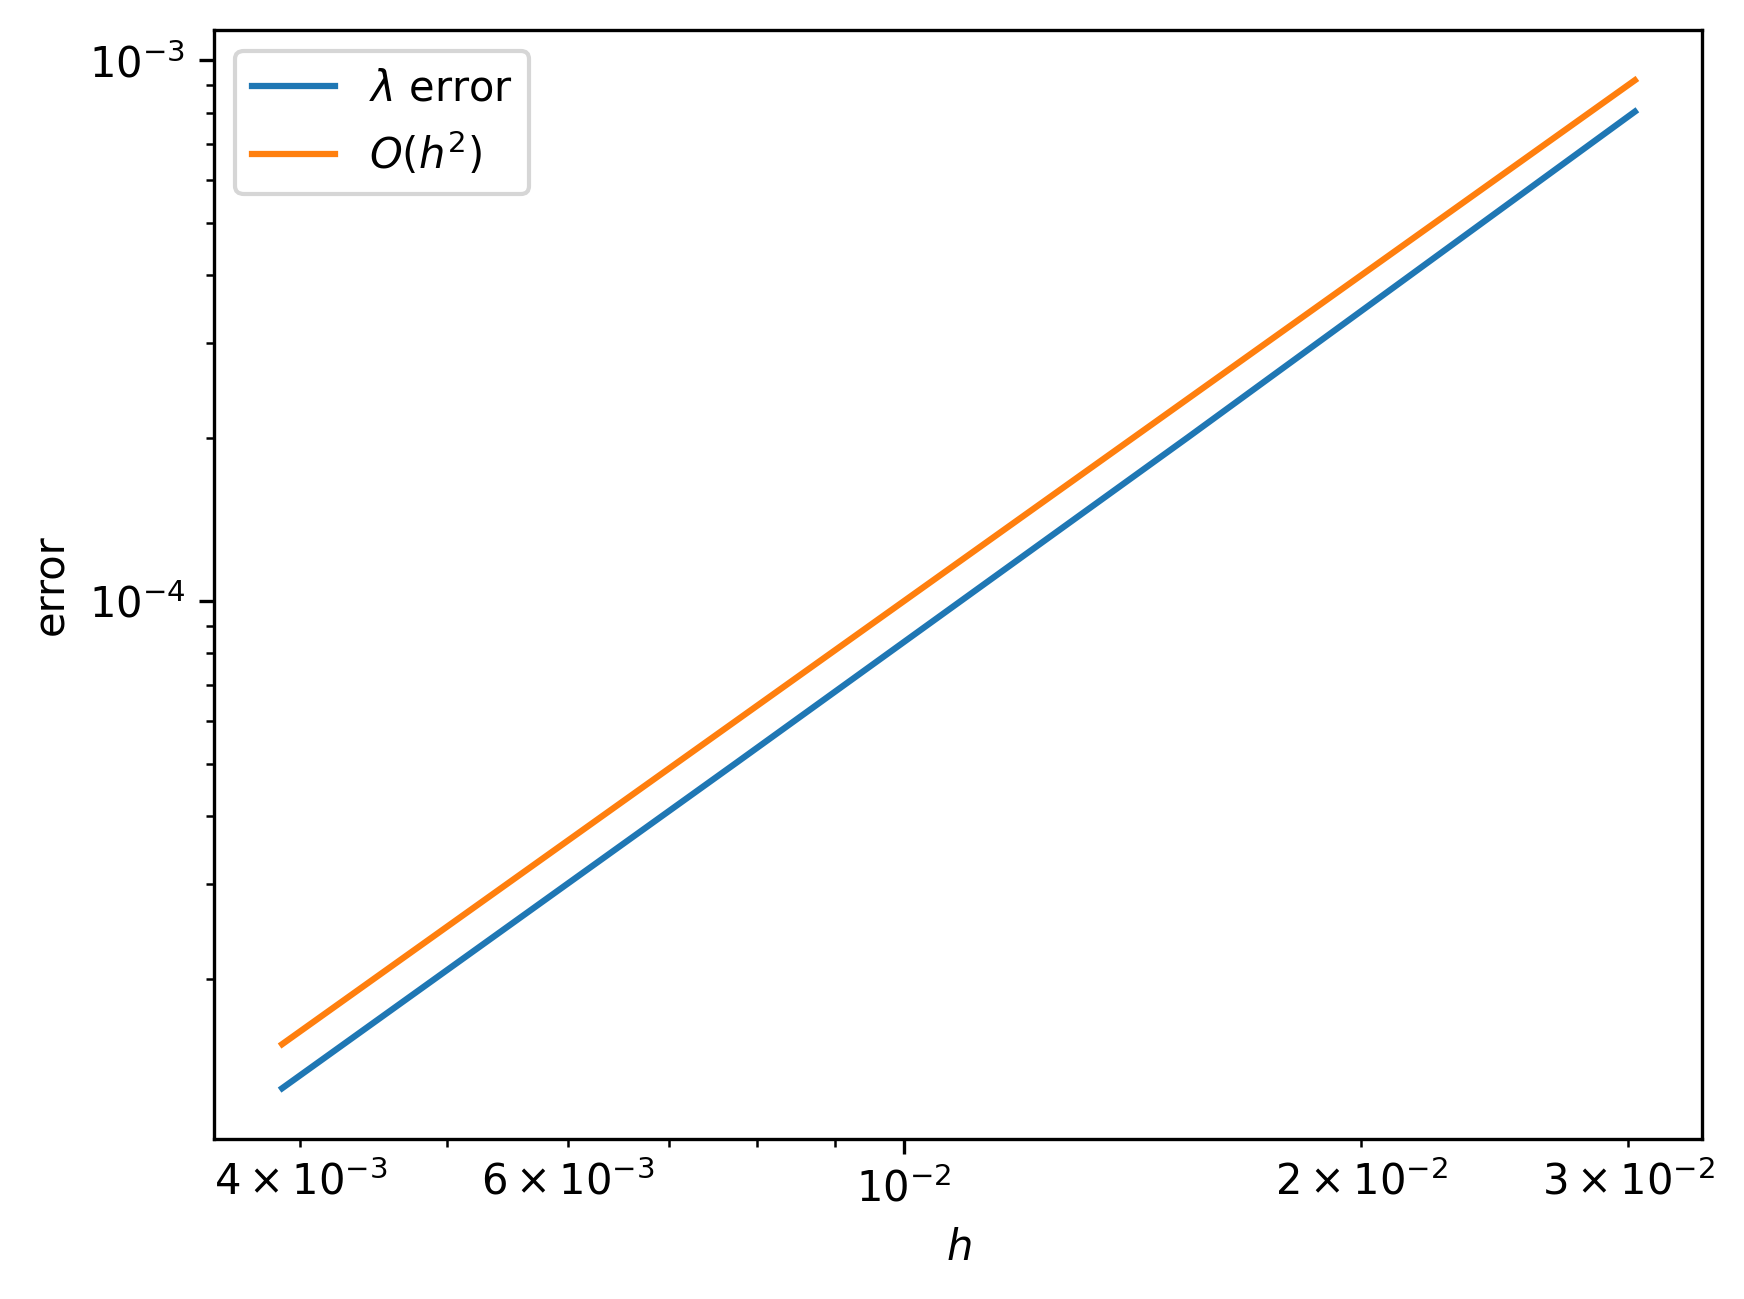
\includegraphics[width=0.5\linewidth]{convergence_test.png}
    \caption{Convergence test for the $1$D Laplace eigenvalue problem. The plot is a log-log plot of the absolute error in the smallest eigenvalue computed using piecewise linear elements on a uniform triangular mesh, plotted against the number of mesh elements $N$ (the mesh has $N \times N$ elements). As expected, we observe approximately second-order convergence.}
    \label{conv test}
\end{figure}


We note that in this setting, the eigenvalues are approximated from above:
\begin{equation}
\lambda^{(k)} \le \lambda_h^{(k)} \le \lambda^{(k)} + C(k) \, h^2.
\end{equation}
Furthermore, since the eigenmodes are unique up to scalar multiples, we need to be careful when computing $\| u^{(k)}  - u_h^{(k)} \|_V.$ To overcome this issue, we first normalize the computed eigenmode. To overcome any sign discrepancies, we choose the sign to match the sign of $u^{(k)}$ (ensure the scalar product of $u^{(k)}$ and $u_h^{(k)}$ is positive).


Now, let $V_h$ be the space of continuous piecewise polynomials of degree at most $p$ that vanish at the endpoints of the interval (standard conforming $P^p$ elements). Then, our convergence results are \cite{boffi}
\begin{equation}
    \| u^{(k)}  - u_h^{(k)} \|_V = O(h^p)
\end{equation}
and
\begin{equation}
    | \lambda^{(k)} - \lambda_h^{(k)} | = O(h^{2p}).
\end{equation}

\subsection{On a Square Domain}

Let $\Omega = (0, \pi) \times (0, \pi).$ We want to find the eigenvalues $\lambda$ and the eigenfunctions $u \ne 0$ such that
\begin{equation}\label{strong 2D}
\begin{aligned}
    - \nabla^2 u &= \lambda u, \qquad (x,y) \in \Omega,\\
    u &= 0 \qquad \forall \, (x, y) \in \partial \Omega.
\end{aligned}
\end{equation}
Here, the exact eigenvalues are
\begin{equation}
\lambda_{m,n} = m^2 + n^2,
\end{equation}
with eigenfunctions
\begin{equation}
u_{m,n} = \sin(mx) \sin(ny), 
\end{equation}
for $m, n \in \mathbb{N}_1$ \cite{boffi}.


Let $V = H_0^1(\Omega).$ As before, the variational formulation of \eqref{strong 2D} is: find a $\lambda \in \mathbb{R}$ and a nonzero $u \in V$ such that
\begin{equation}
\int_{\Omega} \nabla u \cdot \nabla v \, dx dy = \lambda \int_{\Omega} u v \, dxdy,
\end{equation}
for all $v \in V.$


To discretize, we solve for a solution in a finite-dimensional subspace $V_h \subset V,$ namely, the space of continuous piecewise linear finite elements. Thus, we want to find a $\lambda_h \in \mathbb{R}$ and a nonzero $u_h \in V_h$ such that
\begin{equation}
    \int_{\Omega} \nabla u_h \cdot \nabla v \, dx dy = \lambda_h \int_{\Omega} u_h v \, dxdy, 
\end{equation}
for all $v \in V_h.$




As in one dimension, the eigenvalues are approximated from above. Similarly, in one dimension we saw that $| \lambda^{(k)} - \lambda_h^{(k)} | = O(k^4 h^2).$ Thus, the error increases with the rank of the eigenvalues \cite{boffi}. This is again observed in two dimensions.

Consider the double eigenvalue $\lambda = 5,$ whose eigenspace is two-dimensional. The numerical method will approximate $\lambda = 5$ twice, with two eigenmodes $u_h^{(1)}$ and $u_h^{(2)}$. However, because the exact eigenspace is two-dimensional, the computed eigenmodes need not converge to the particular basis functions, say $u_1$ and $u_2.$ Rather, they can converge to any linear combination of $u_1$ and $u_2.$ 

Therefore, for multiple eigenvalues, to compute the error in the computed eigenmodes, we compare the computed eigenspace to the exact eigenspace rather than the individual eigenfunctions. For example, for $\lambda = 5$, we expect constants $\alpha_1(h),$ $\alpha_2(h),$ $\beta_1(h),$ and $\beta_2(h)$ such that
\begin{equation}
    \| u_{1} - \alpha_1(h) \,u_h^{(1)} - \beta_1 \, (h) u_h^{(2)} \|_{V} = O(h)
\end{equation}
and
\begin{equation}
   \| u_{2} - \alpha_2(h)\, u_h^{(1)} - \beta_2(h)\, u_h^{(2)} \|_{V} = O(h), 
\end{equation}
where $h$ is the maximum diameter of any element of the mesh\footnote{Is this the correct definition of $h$ in this context?} \cite{boffi}. The dependence of $\alpha_1(h),$ $\alpha_2(h),$ $\beta_1(h),$ and $\beta_2(h)$ on the mesh 
reflects the nonuniqueness of the computed eigenbasis for a multiple eigenvalue. In particular, as the mesh varies, the computed eigenmodes may converge to different linear combinations of $u_1$ and $u_2.$  

To illustrate this mesh-dependence, we first approximate the eigenvalues and eigenfunctions of \eqref{strong 2D} on a sequence of unstructured meshes. These results are shown in Figure \ref{unstructured}. 

\begin{figure}[htbp]
    \centering

    \begin{subfigure}{1.0\textwidth}
        \centering
        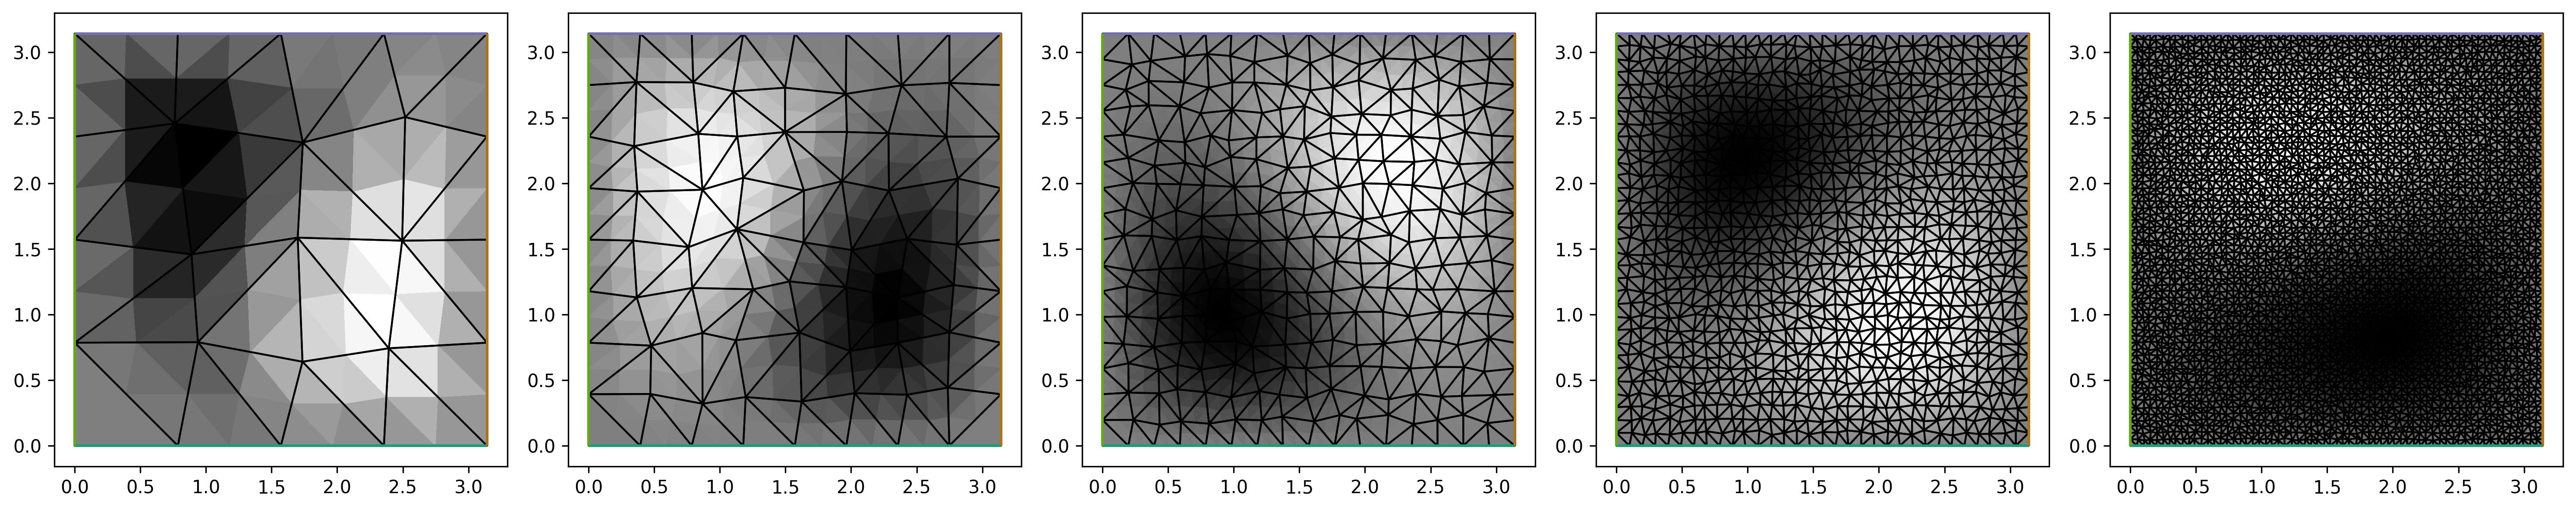
\includegraphics[width=\textwidth]{unstructured_u1h.png}
        \caption{Computed eigenmodes for the first approximation of $\lambda = 5$ on an unstructured mesh sequence.}
        \label{fig:diag-one}
    \end{subfigure}

    \vspace{1em}

    \begin{subfigure}{1.0\textwidth}
        \centering
        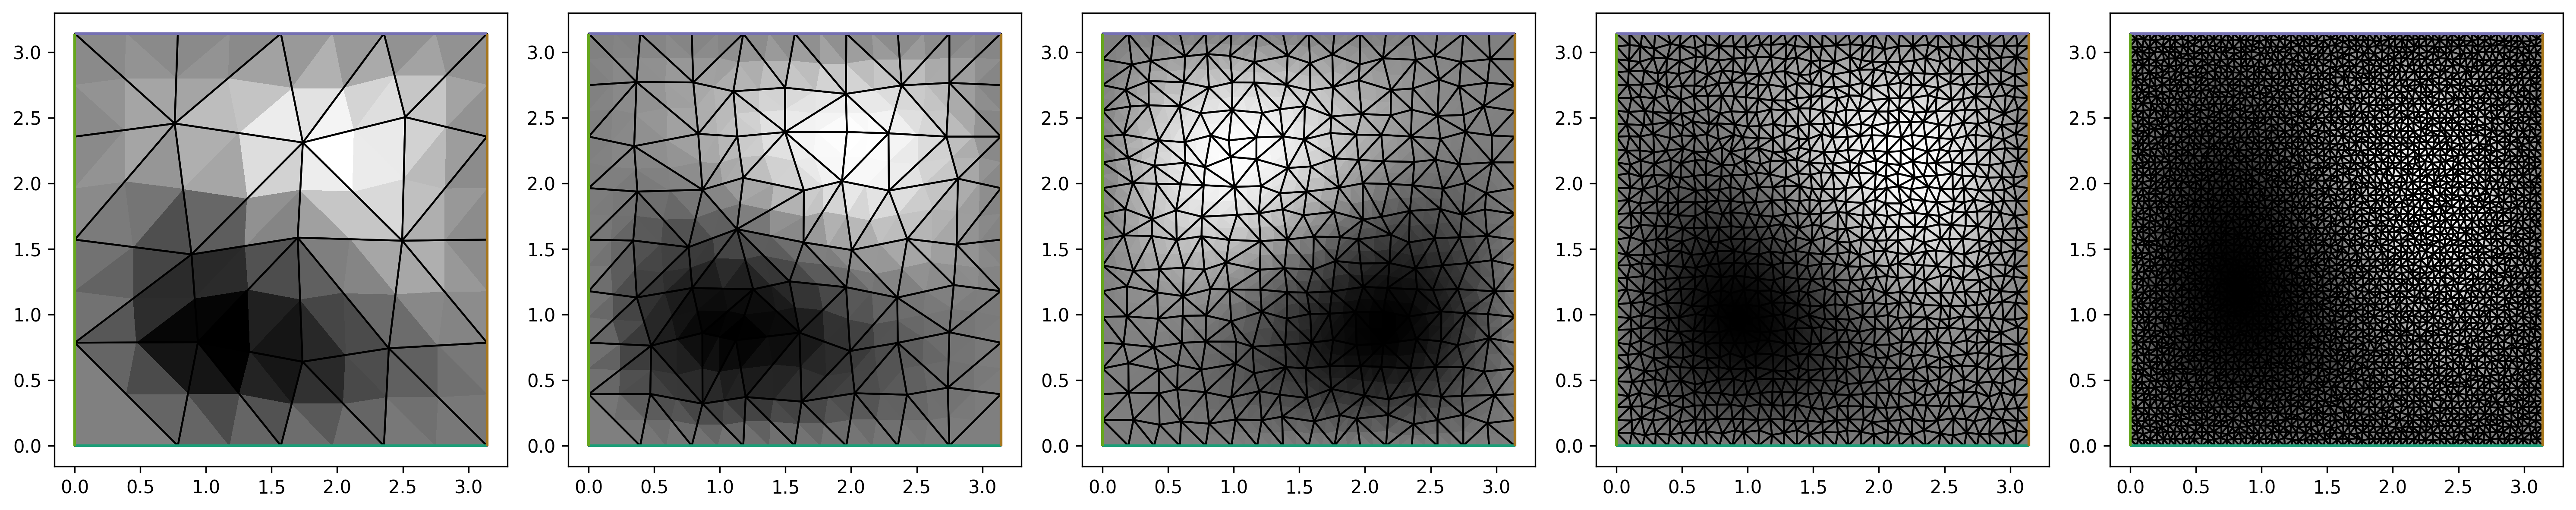
\includegraphics[width=\textwidth]{unstructured_u2h_png.png}
        \caption{Computed eigenmodes for the second approximation of $\lambda = 5$ on an unstructured mesh sequence.}
        \label{fig:diag-two}
    \end{subfigure}

    \vspace{1em}

    \begin{subfigure}{0.4\textwidth}
        \centering
        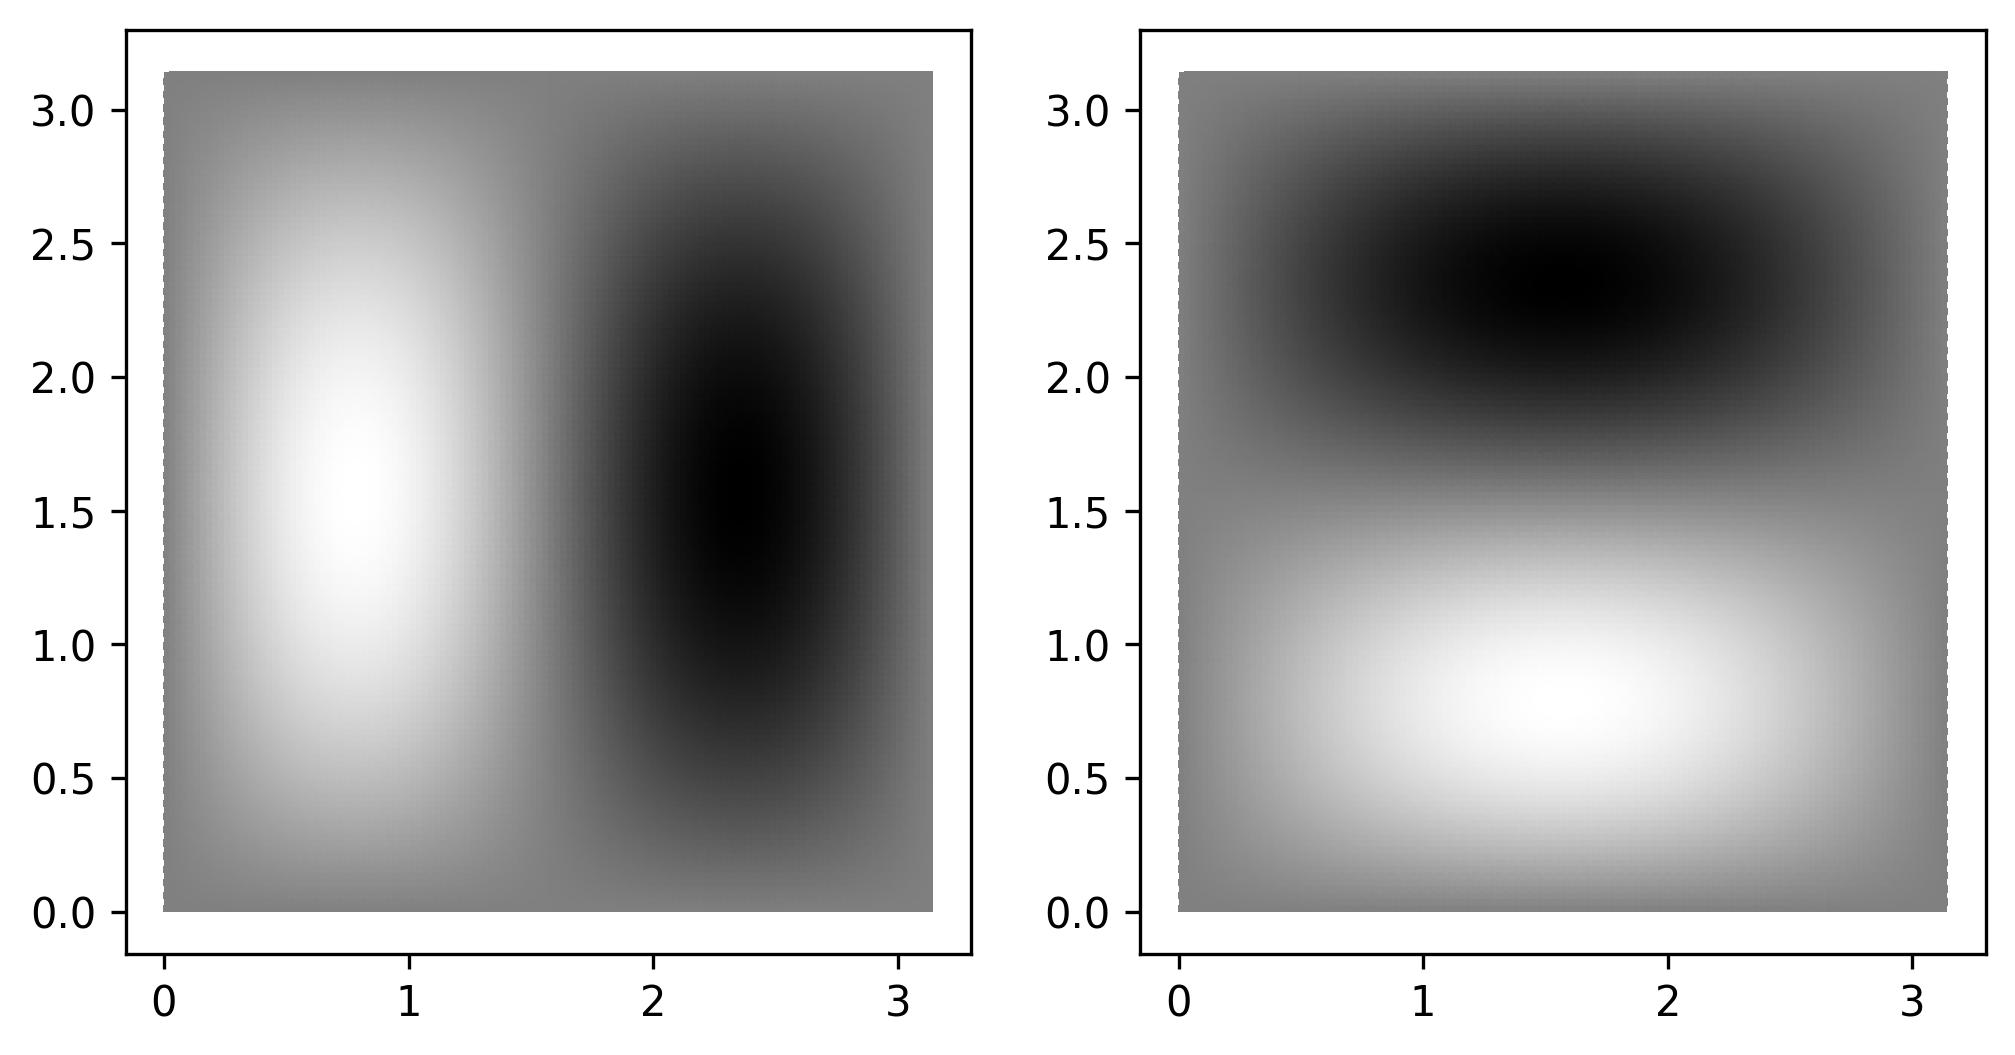
\includegraphics[width=\textwidth]{unstructured_u12.png}
        \caption{The exact eigenfunctions.}
        \label{fig:eigenfunction-comparison}
    \end{subfigure}

    \caption{The computed eigenmodes for both approximations of $\lambda = 5$ on sequences of unstructured meshes.}
    \label{unstructured}
\end{figure}

The situation is similar for structured uniform meshes, where we see an improvement in the computed convergence rates because the mesh is uniform. The results are shown in Figure \ref{structured}, where the computed eigenmodes are visibly influenced by the preferred diagonal direction of the mesh \cite{boffi}.

\begin{figure}[htbp]
    \centering

    \begin{subfigure}{1.0\textwidth}
        \centering
        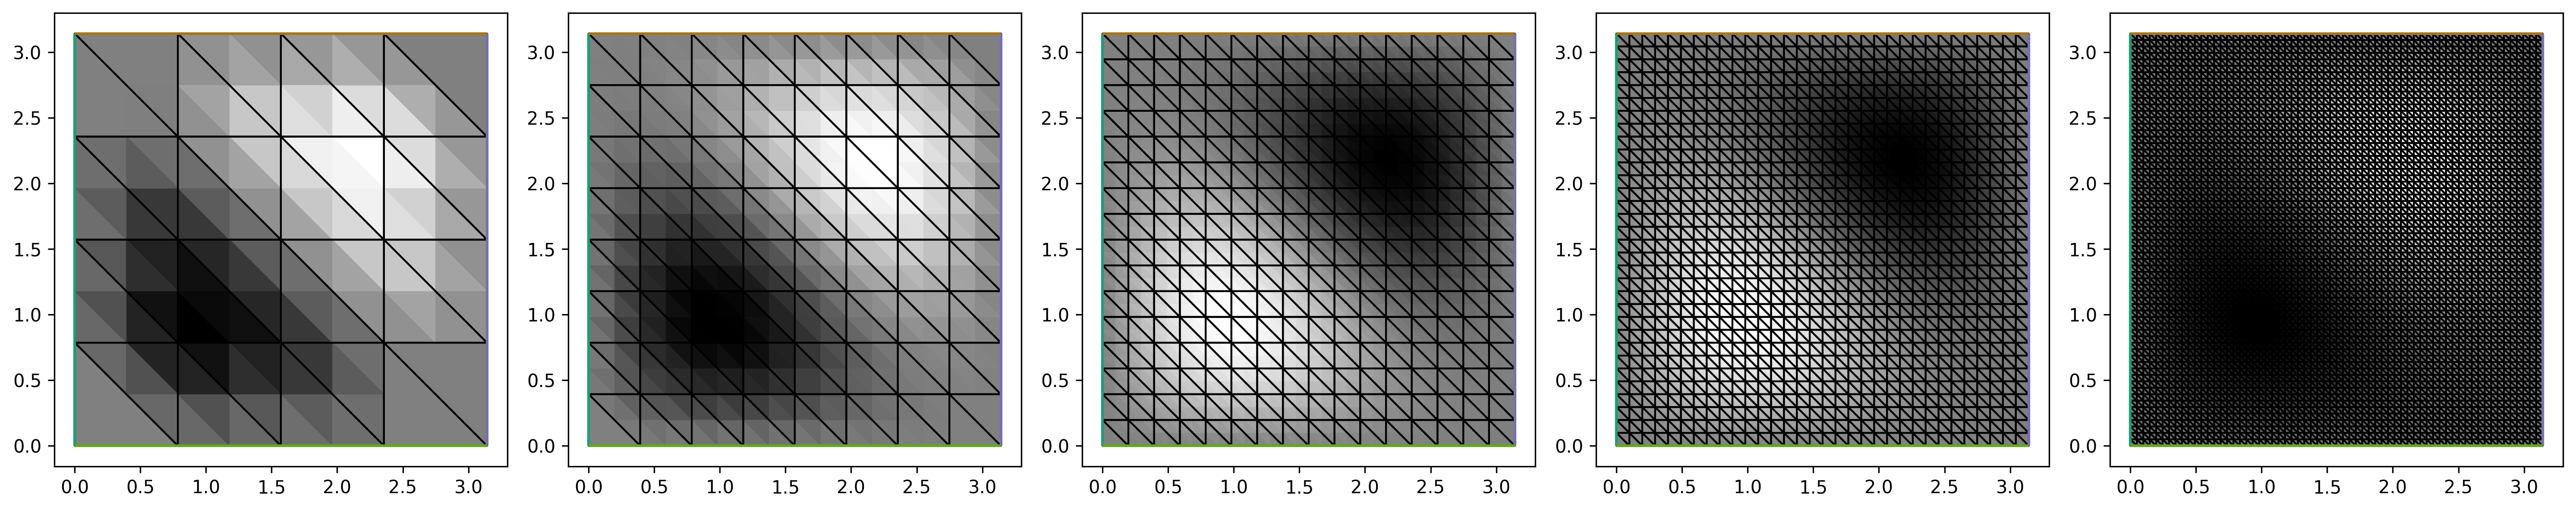
\includegraphics[width=\textwidth]{structured_u1h.png}
        \caption{Computed eigenmodes for the first approximation of $\lambda = 5$ on a uniform structured mesh sequence.}
        \label{fig:diag-one}
    \end{subfigure}

    \vspace{1em}

    \begin{subfigure}{1.0\textwidth}
        \centering
        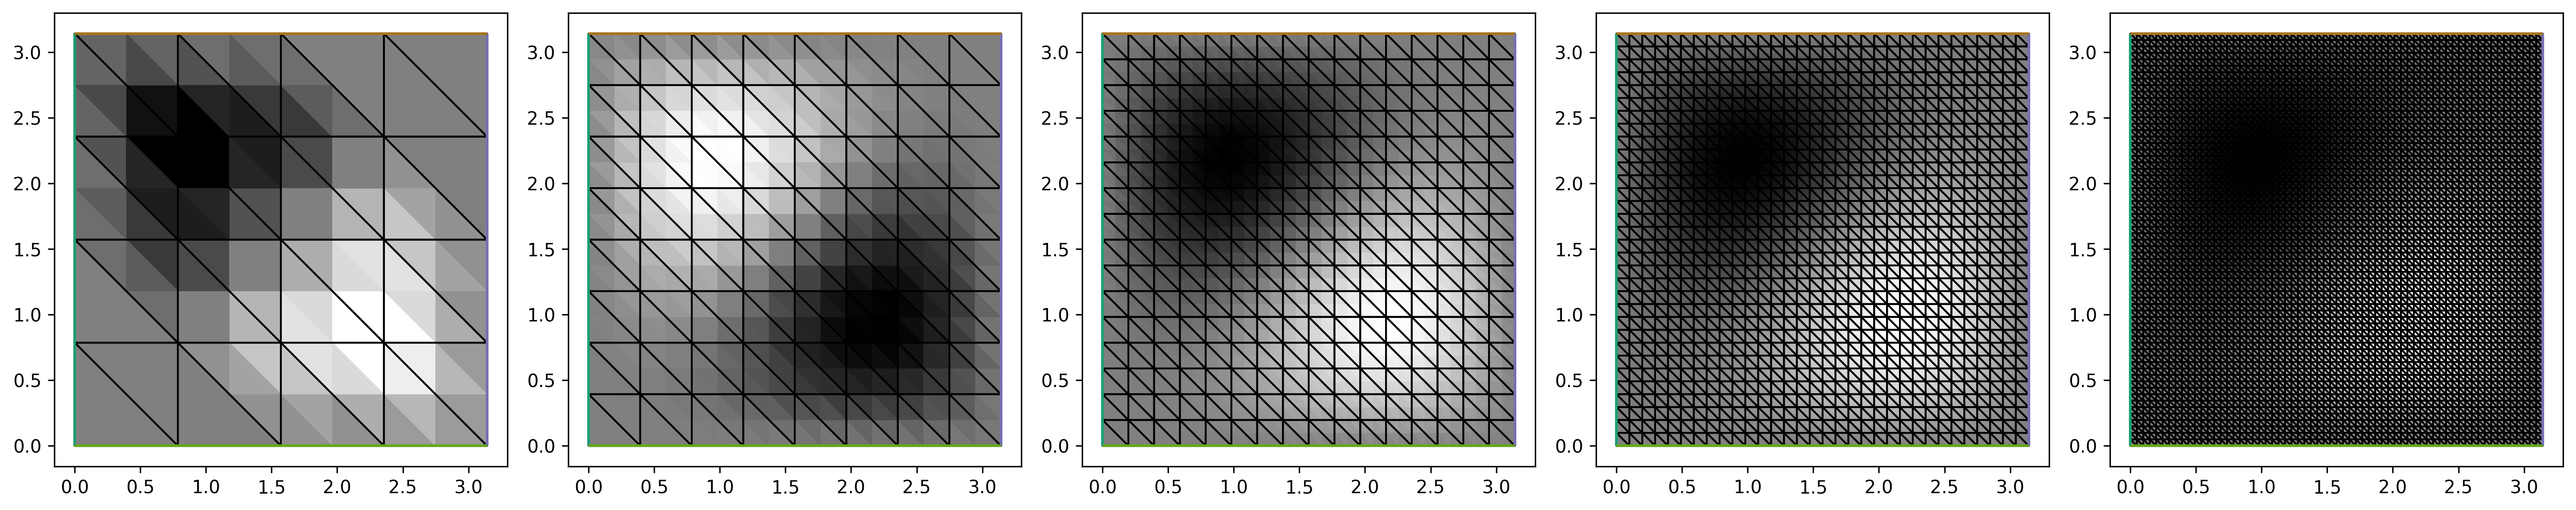
\includegraphics[width=\textwidth]{structured_u2h.png}
        \caption{Computed eigenmodes for the second approximation of $\lambda = 5$ on a unfiorm structured mesh sequence.}
        \label{fig:diag-two}
    \end{subfigure}

    % \vspace{1em}

    % \begin{subfigure}{0.4\textwidth}
    %     \centering
    %     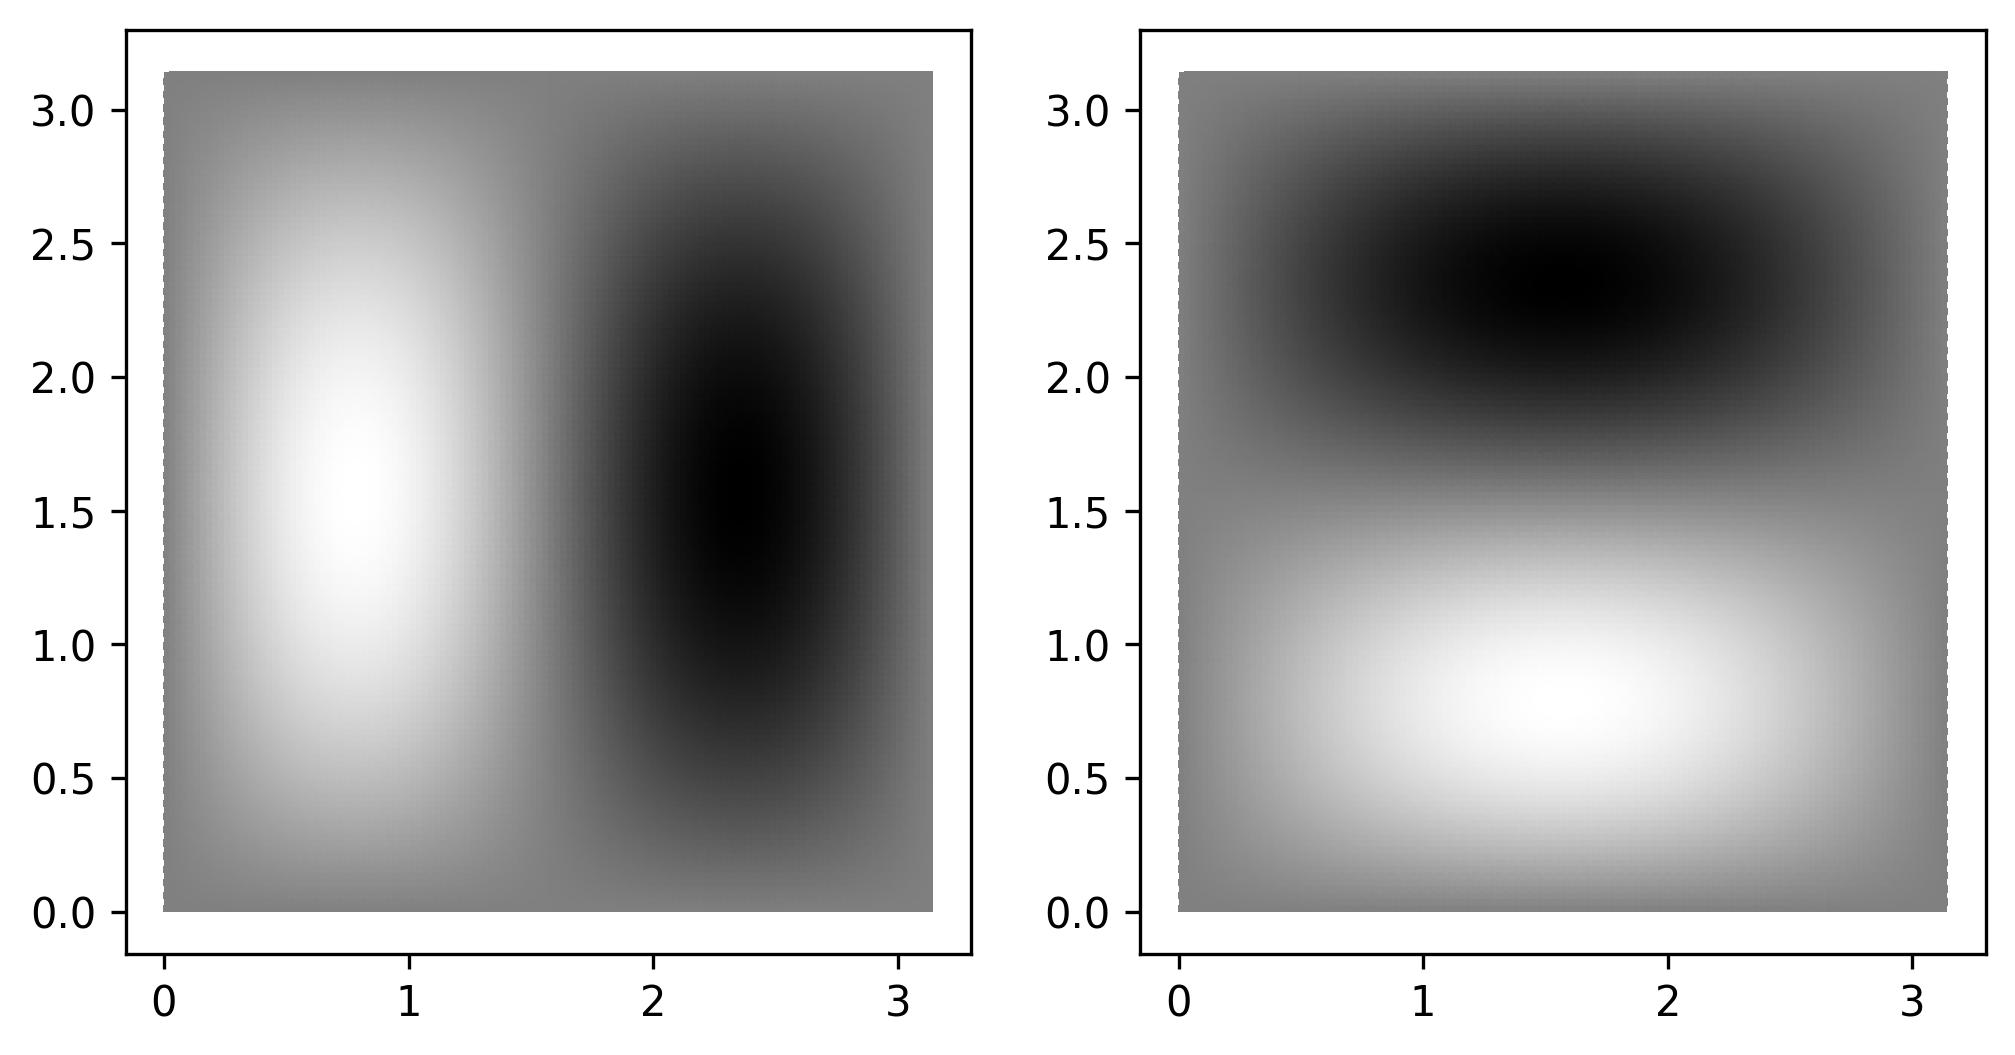
\includegraphics[width=\textwidth]{structured_u12.png}
    %     \caption{The exact eigenfunctions.}
    %     \label{fig:eigenfunction-comparison}
    % \end{subfigure}

    \caption{The computed eigenmodes for both approximations of $\lambda = 5$ on sequences of uniform structured meshes.}
    \label{structured}
\end{figure}



To further explore this mesh-dependence, we take another uniform grid, but now cut each square along the opposite diagonal direction. The eigenvalues are the same as before. 
However, as shown in Figure \ref{reverse}, the eigenfunctions change. This behaviour change is attributed to the change in the preferred diagonal direction of the mesh \cite{boffi}. As a result, the discrete problem selects different linear combinations inside the same eigenspace. This result is not surprising since the problem is invariant under the change of variables induced by the symmetry about the line $y=\pi-x$ \cite{boffi}.
% This result is expected since the new mesh is just a reflected/rotated version of the old one.

\begin{figure}[htbp]
    \centering

    \begin{subfigure}{1.0\textwidth}
        \centering
        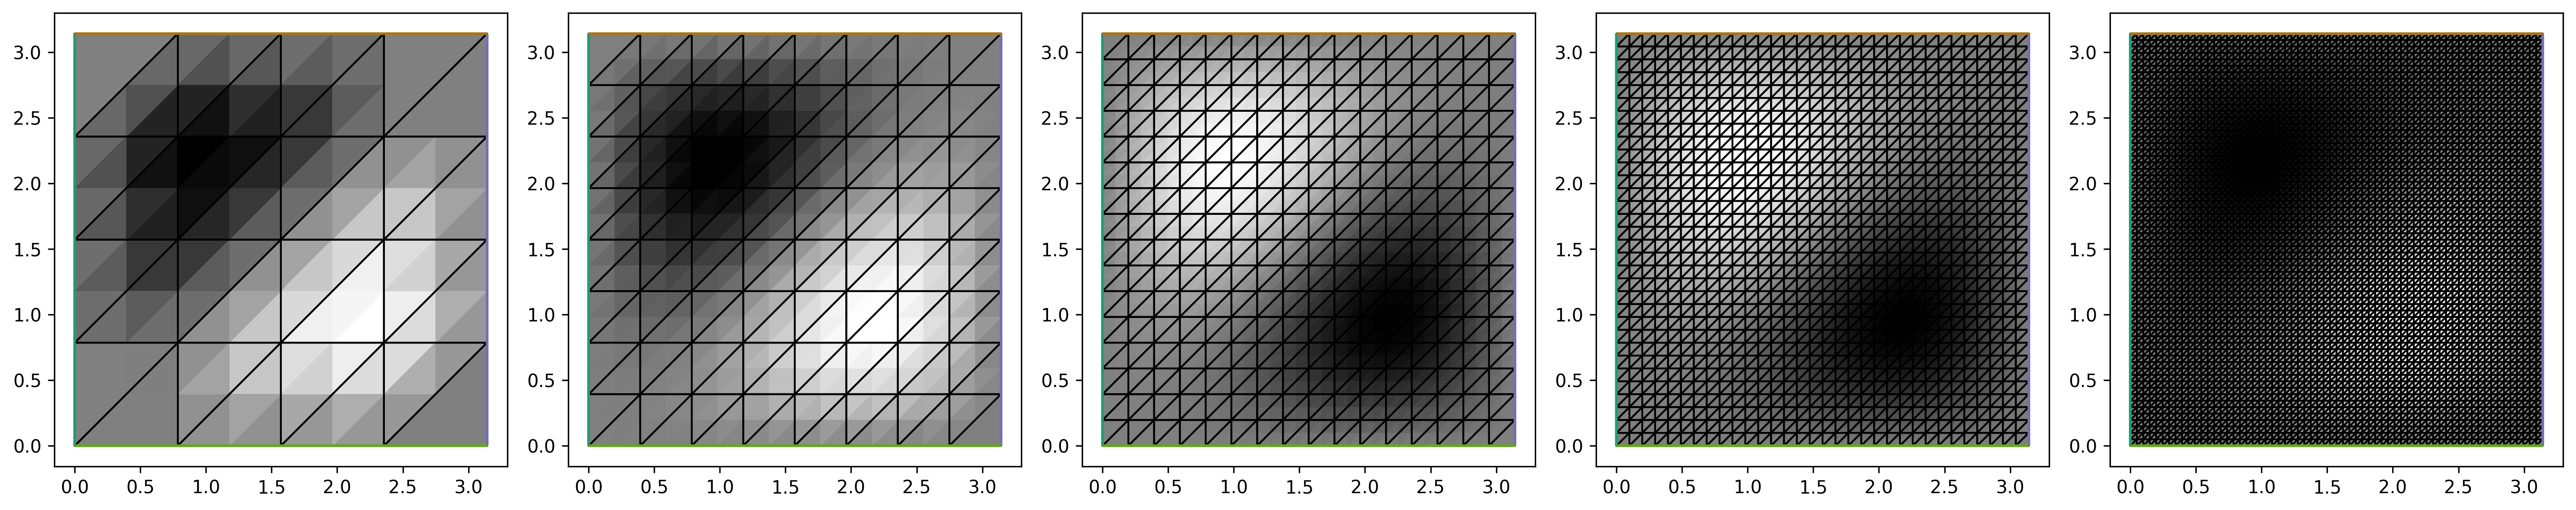
\includegraphics[width=\textwidth]{reverse_u1h.png}
        \caption{Computed eigenmodes for the first approximation of $\lambda = 5$ on a uniform structured mesh sequence (reverse orientation).}
        \label{fig:diag-one}
    \end{subfigure}

    \vspace{1em}

    \begin{subfigure}{1.0\textwidth}
        \centering
        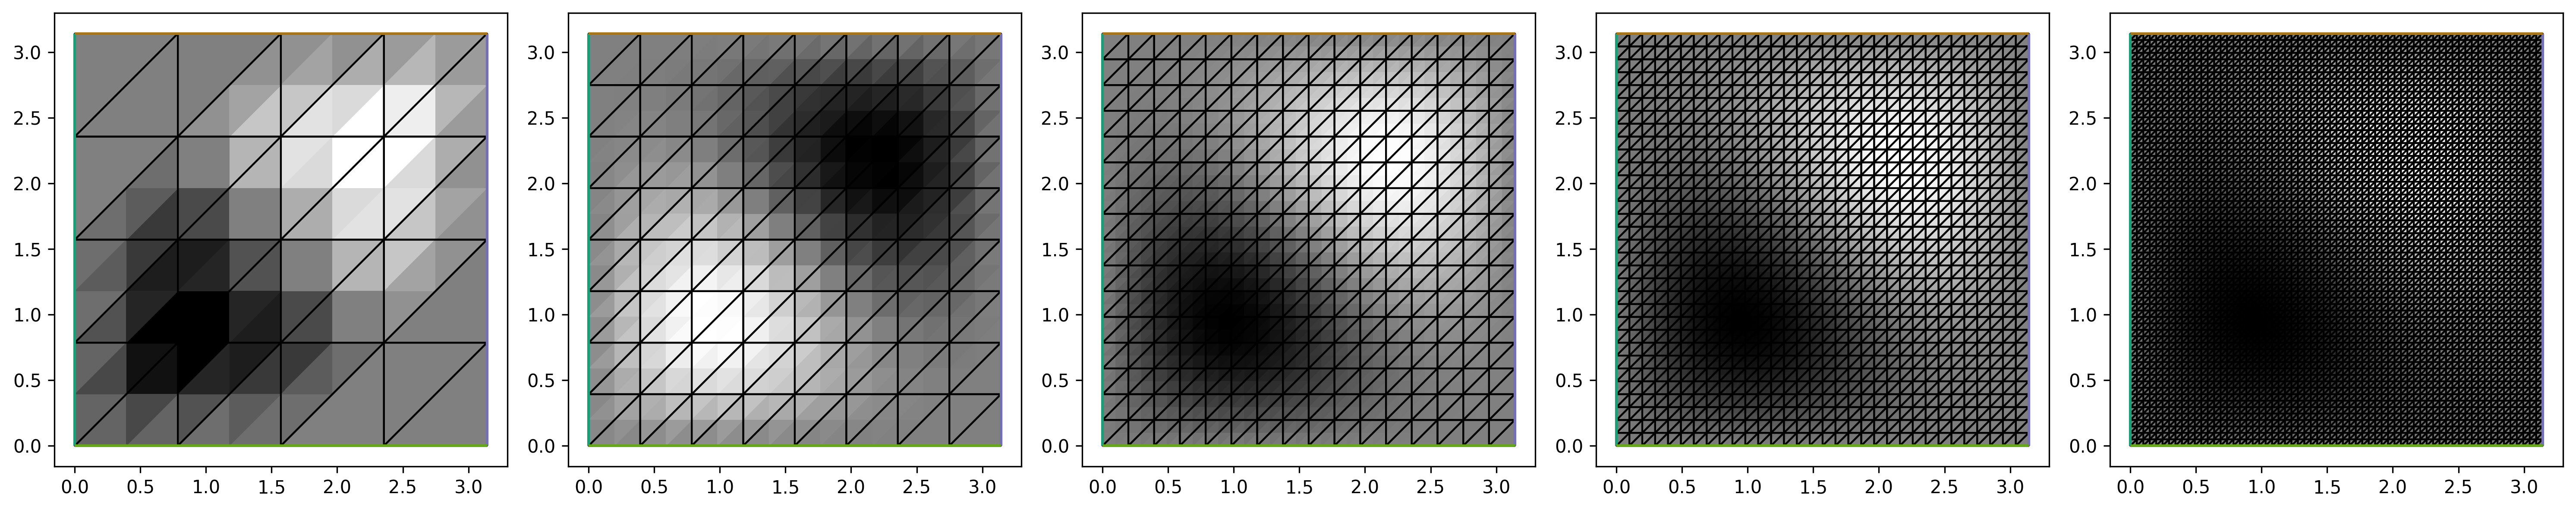
\includegraphics[width=\textwidth]{reverse_u2h.png}
        \caption{Computed eigenmodes for the second approximation of $\lambda = 5$ on a unfiorm structured mesh sequence (reverse orientation).}
        \label{fig:diag-two}
    \end{subfigure}

    % \vspace{1em}

    % \begin{subfigure}{0.4\textwidth}
    %     \centering
    %     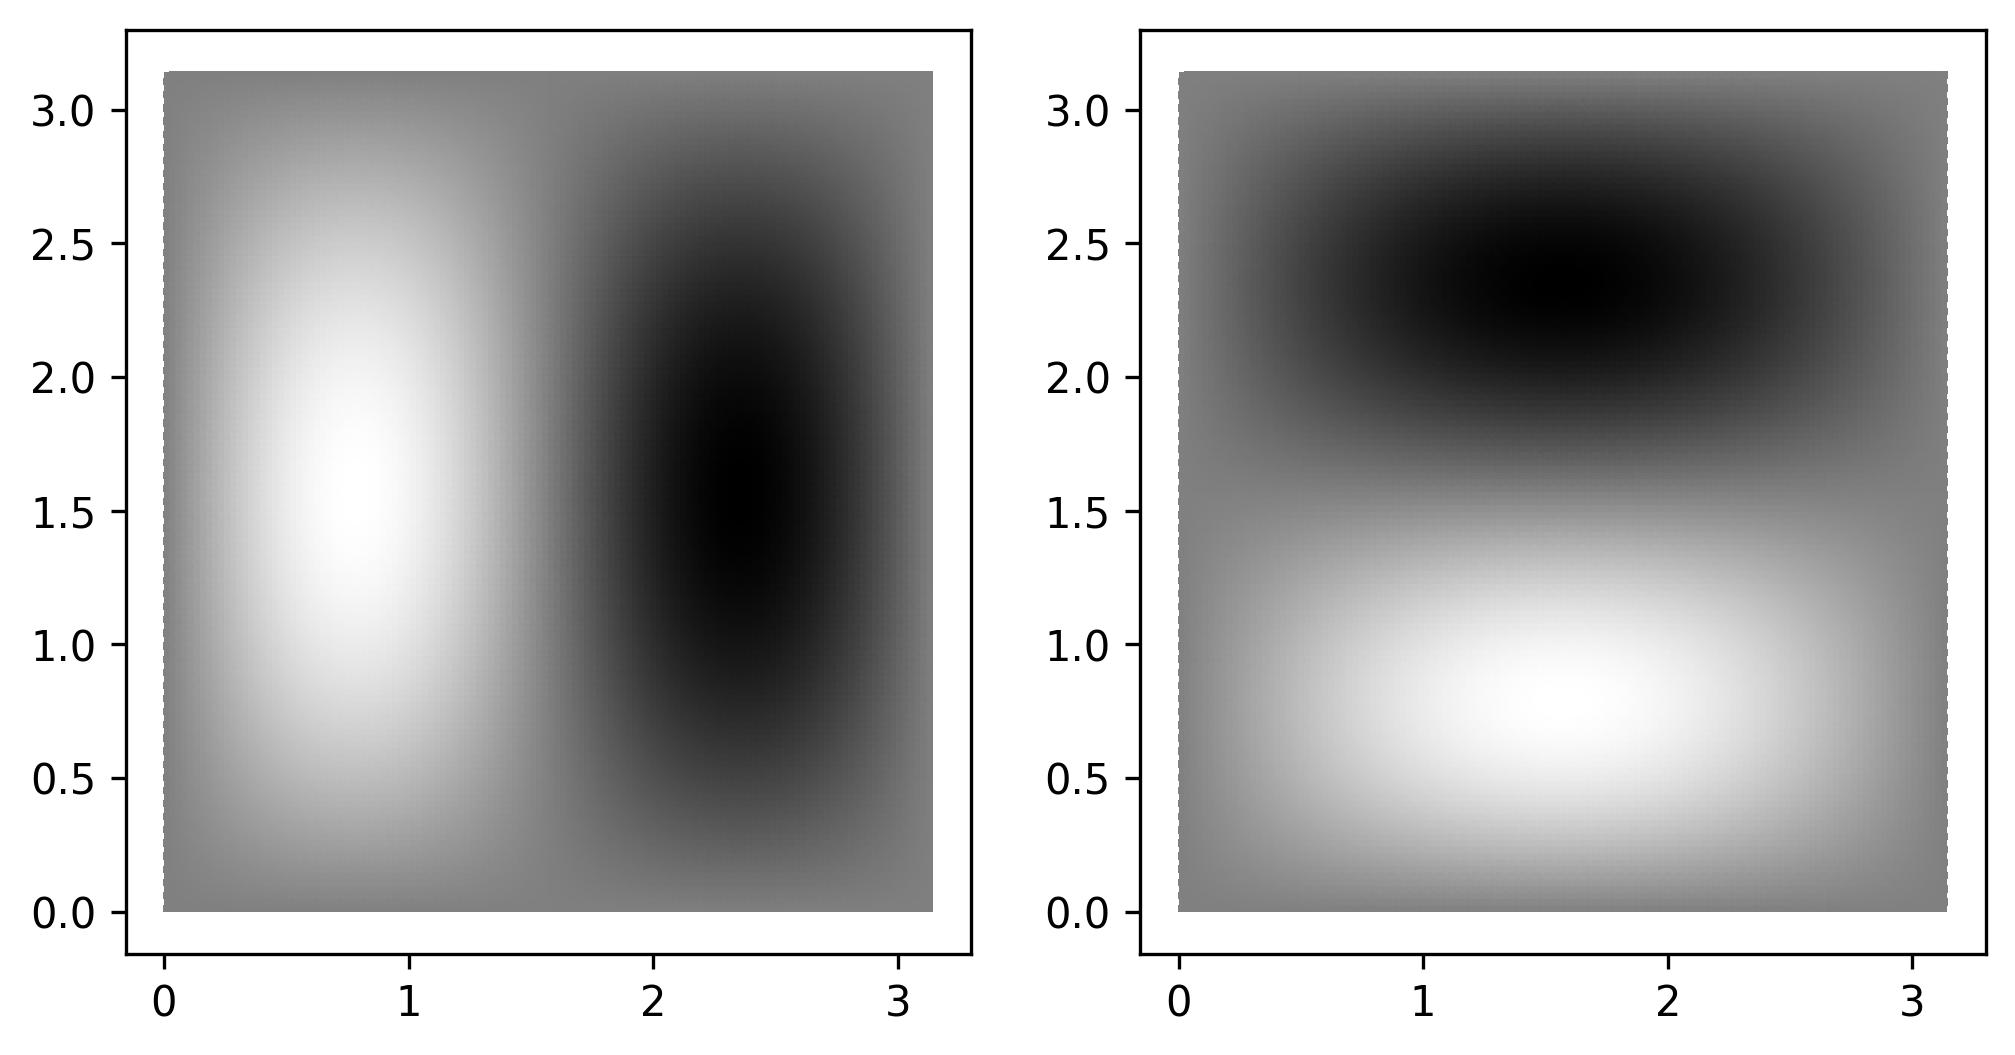
\includegraphics[width=\textwidth]{reverse_u12.png}
    %     \caption{The exact eigenfunctions.}
    %     \label{fig:eigenfunction-comparison}
    % \end{subfigure}

    \caption{The computed eigenmodes for both approximations of $\lambda = 5$ on sequences of uniform structured meshes (reverse orientation).}
    \label{reverse}
\end{figure}

Next, we consider a sequence of criss-cross meshes. The results of this example are shown in Table \ref{table criss cross}. Notice that the additional symmetry of these meshes manifests as coinciding approximations of some of the repeated eigenvalues. For example, $\lambda = 5,$ $\lambda = 10,$ and $\lambda = 13$ are approximated by discrete eigenvalues that are the same up to machine precision. However, this is not the case for the approximations of $\lambda = 17$ on the coarsest mesh. This occurs because the ninth computed eigenvalue, $\lambda_h^{(9)},$ is a bad approximation of $\lambda = 18$ instead of $\lambda = 17$ \cite{boffi}. This is supported by the comparison between the computed eigenmode for $\lambda_h^{(9)}$ and the exact eigenfunction for $\lambda = 18$ in Figure \ref{compare}. Thus, this example should be taken as a cautionary tale: when the discretization is too coarse, the order of the computed eigenvalues need not be in one-to-one correspondence with the exact eigenvalues.

% \begin{table}[htbp]
\begin{table}[htbp]
\centering
\caption{Computed eigenvalues on the sequence of criss-cross meshes. Given in parentheses are the observed convergence rates. Note that I have not explained what $N$ is!}
\label{table criss cross}
\resizebox{\textwidth}{!}{%
\begin{tabular}{c|ccccc}
\toprule
Exact & \multicolumn{5}{c}{Computed (rate)} \\
\cmidrule(lr){2-6}
 & $N=4$ & $N=8$ & $N=16$ & $N=32$ & $N=64$ \\
\midrule
$2$  & $2.0880$  & $2.0216\ (2.0)$  & $2.0054\ (2.0)$  & $2.0013\ (2.0)$  & $2.0003\ (2.0)$ \\
$5$  & $5.6811$  & $5.1651\ (2.0)$  & $5.0408\ (2.0)$  & $5.0102\ (2.0)$  & $5.0025\ (2.0)$ \\
$5$  & $5.6811$  & $5.1651\ (2.0)$  & $5.0408\ (2.0)$  & $5.0102\ (2.0)$  & $5.0025\ (2.0)$ \\
$8$  & $9.4962$  & $8.3521\ (2.1)$  & $8.0863\ (2.0)$  & $8.0215\ (2.0)$  & $8.0054\ (2.0)$ \\
$10$ & $12.9691$ & $10.7578\ (2.0)$ & $10.1865\ (2.0)$ & $10.0464\ (2.0)$ & $10.0116\ (2.0)$ \\
$10$ & $12.9691$ & $10.7578\ (2.0)$ & $10.1865\ (2.0)$ & $10.0464\ (2.0)$ & $10.0116\ (2.0)$ \\
$13$ & $17.1879$ & $14.0237\ (2.0)$ & $13.2489\ (2.0)$ & $13.0617\ (2.0)$ & $13.0154\ (2.0)$ \\
$13$ & $17.1879$ & $14.0237\ (2.0)$ & $13.2489\ (2.0)$ & $13.0617\ (2.0)$ & $13.0154\ (2.0)$ \\
$17$ & $25.1471$ & $19.3348\ (1.8)$ & $17.5733\ (2.0)$ & $17.1423\ (2.0)$ & $17.0355\ (2.0)$ \\
$17$ & $38.9073$ & $19.3348\ (3.2)$ & $17.5733\ (2.0)$ & $17.1423\ (2.0)$ & $17.0355\ (2.0)$ \\
$18$ & $38.9073$ & $19.8363\ (3.5)$ & $18.4405\ (2.1)$ & $18.1089\ (2.0)$ & $18.0271\ (2.0)$ \\
$20$ & $38.9073$ & $22.7243\ (2.8)$ & $20.6603\ (2.0)$ & $20.1634\ (2.0)$ & $20.0407\ (2.0)$ \\
$20$ & $38.9073$ & $22.7243\ (2.8)$ & $20.6603\ (2.0)$ & $20.1634\ (2.0)$ & $20.0407\ (2.0)$ \\
$25$ & $38.9073$ & $28.7526\ (1.9)$ & $25.8940\ (2.1)$ & $25.2202\ (2.0)$ & $25.0548\ (2.0)$ \\
$25$ & $38.9073$ & $28.7526\ (1.9)$ & $25.8940\ (2.1)$ & $25.2202\ (2.0)$ & $25.0548\ (2.0)$ \\
\midrule
DOF & $25$ & $113$ & $481$ & $1985$ & $8065$ \\
\bottomrule
\end{tabular}%
}
\end{table}



\begin{figure}
    \centering
    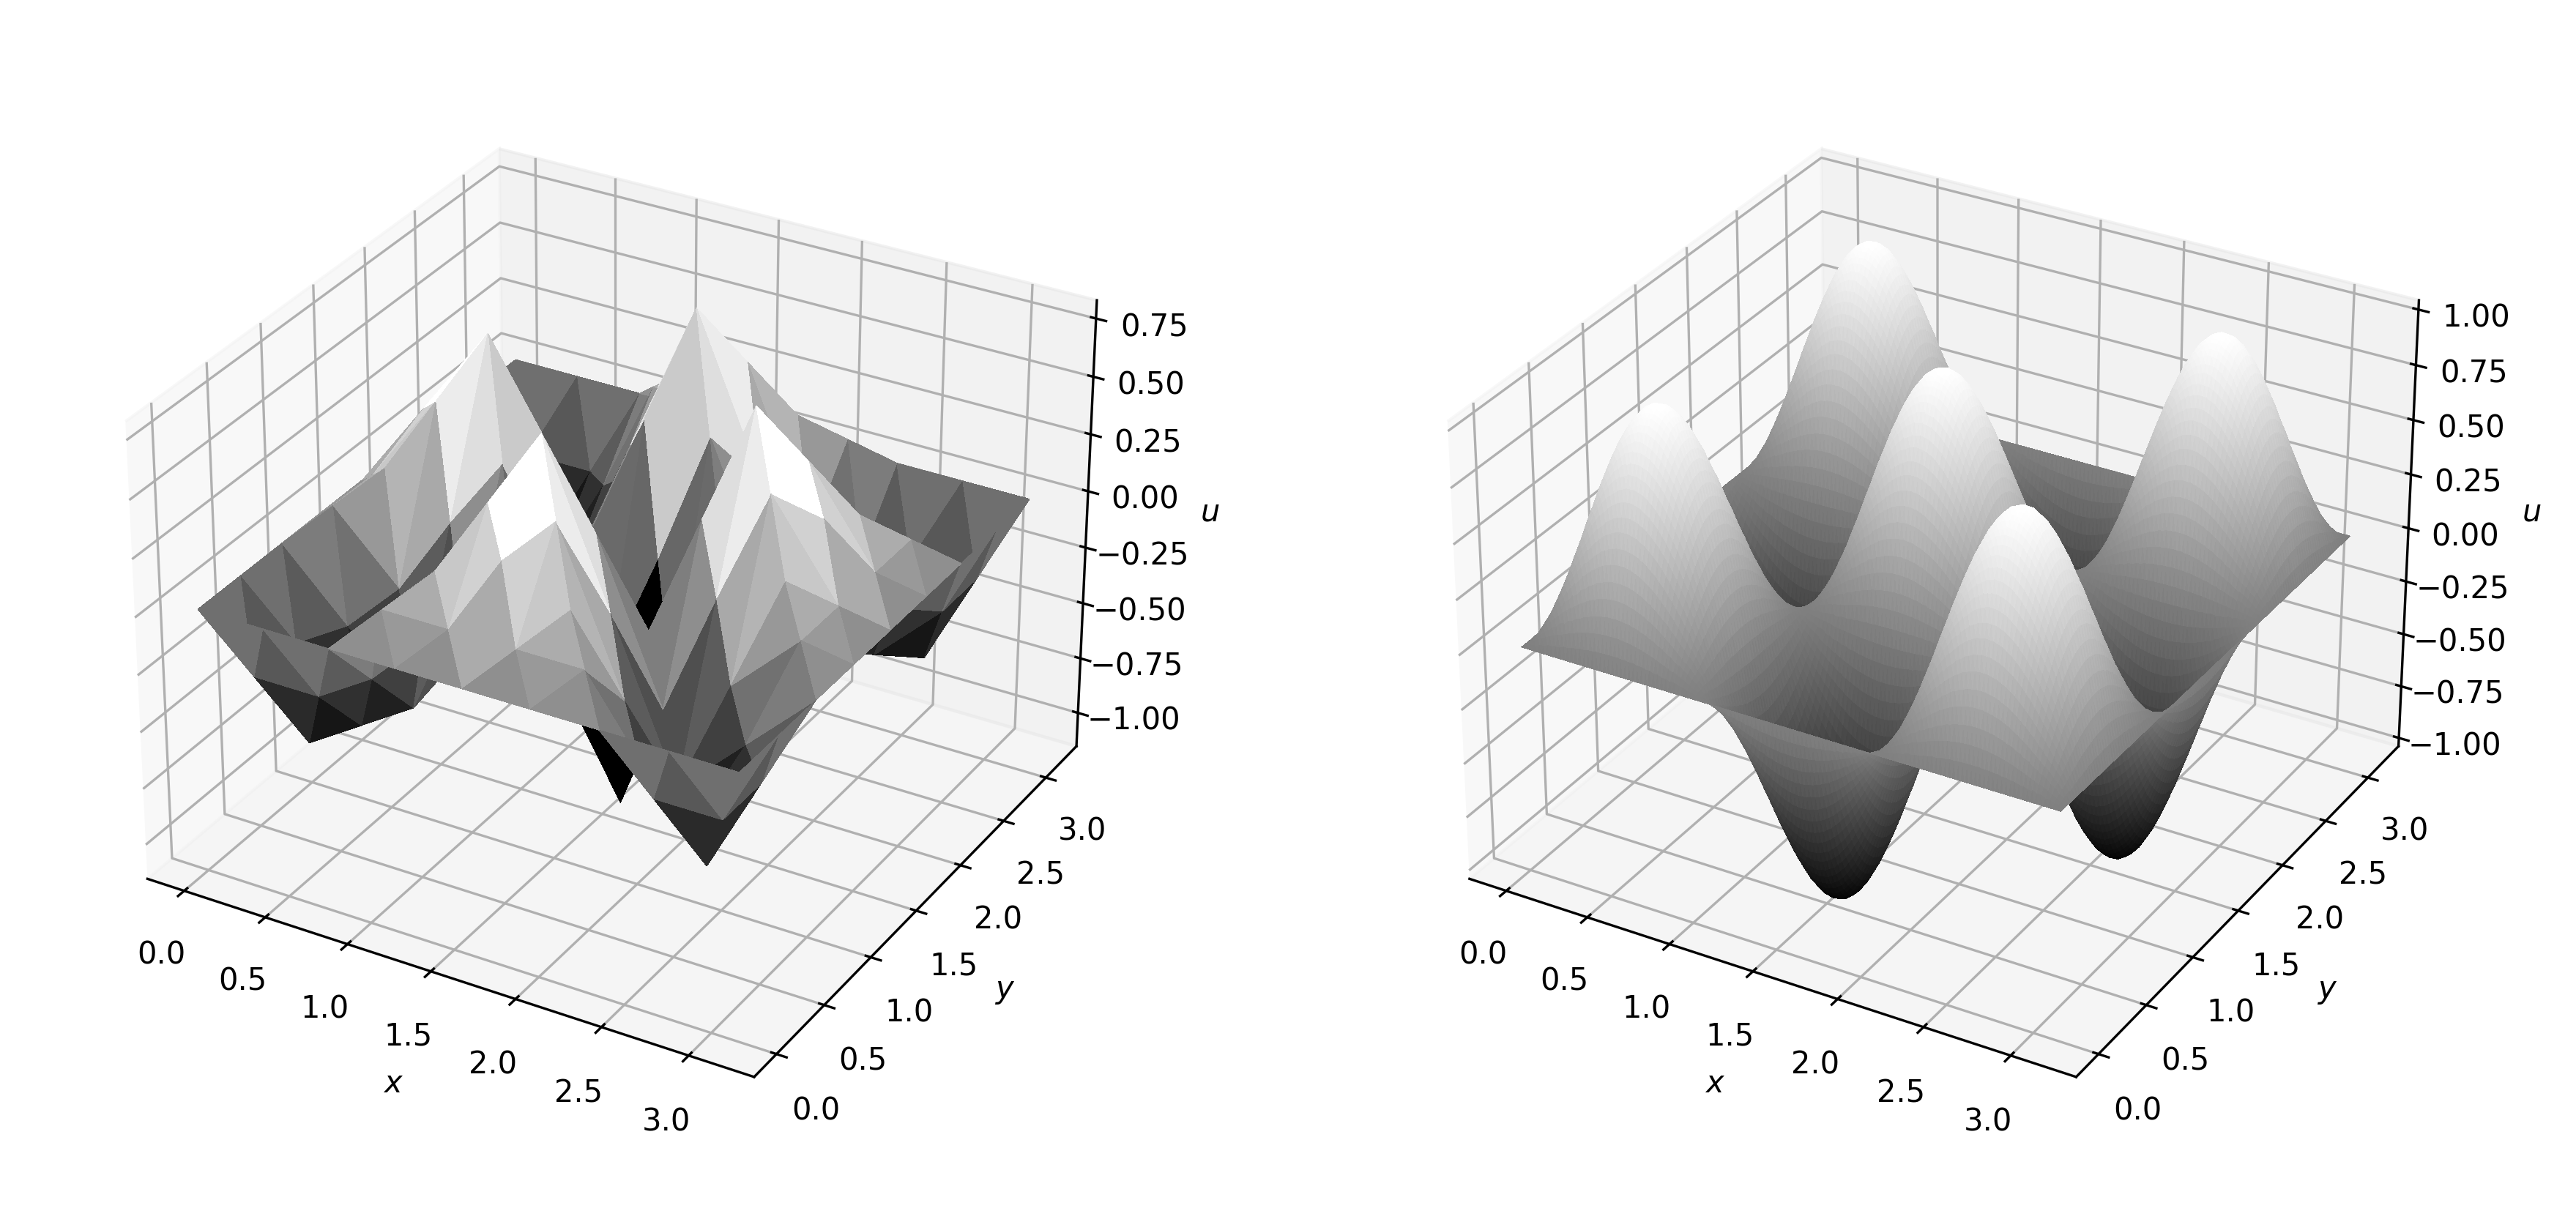
\includegraphics[width=1.0\linewidth]{eigenfunc_comparison.png}
    \caption{Comparing the computed eigenmode for the ninth computed eigenvalue to the exact eigenfunction for $\lambda = 18,$ namely, $u(x, y) = \sin(3x)\sin(3y).$}
    \label{compare}
\end{figure}


\subsection{On an L-Shaped Domain}

Next, we approximate nonsmooth solutions by considering an L-shaped domain. In particular, we consider a domain with a re-entrant corner and a sequence of unstructured meshes. The domain is a flipped L, with coordinates: $(0, 0),$ $ (1, 0),$ $ (1, 1), $ $(-1, 1),$ $ (-1, -1)$ and $(0, -1).$

Here, we solve the Neumann problem:
\begin{equation}
\begin{aligned}
    - \nabla^2 u &= \lambda u, \qquad (x, y) \in \Omega, \\
    \frac{\partial u}{\partial n} &= 0, \qquad \forall(x, y) \in  \, \partial \Omega.
\end{aligned}
\end{equation}
For our experiments, the reference eigenvalues are $\lambda \approx 0, 1.48, 3.53, 9.87, 11.39$ \cite{boffi}.

Consider $V = H^1(\Omega).$ For the variational formulation of the problem, we want to find a $\lambda \in \mathbb{R}$ and a nonzero $u \in V$ such that
\begin{equation}
    \int_{\Omega} \nabla u \cdot \nabla v \, dx dy = \lambda \int_{\Omega} u v \, dxdy
\end{equation}
for all $v \in V.$ As before, we solve for a solution in a finite-dimensionall subspace of $V,$ namely, the space of continuous piecewise linear finite elements. Thus, we want to
find a $\lambda_h \in \mathbb{R}$ and a nonzero $u_h \in V_h$ such that
\begin{equation}
    \int_{\Omega} \nabla u_h \cdot \nabla v \, dx dy = \lambda_h \int_{\Omega} u_h v \, dxdy
\end{equation}
for all $v \in V_h \subset V_h.$


The results obtained on a sequence of unstructured meshes are reported in Table \ref{Lshaped_table}. The corresponding meshes are shown in Figure \ref{Lshape}. As before, the discrete eigenvalues approximate the continuous ones from above. Furthermore, since we are considering a Neumann problem, there is a vanishing frequency (zero eigenvalue).


\begin{figure}
    \centering
    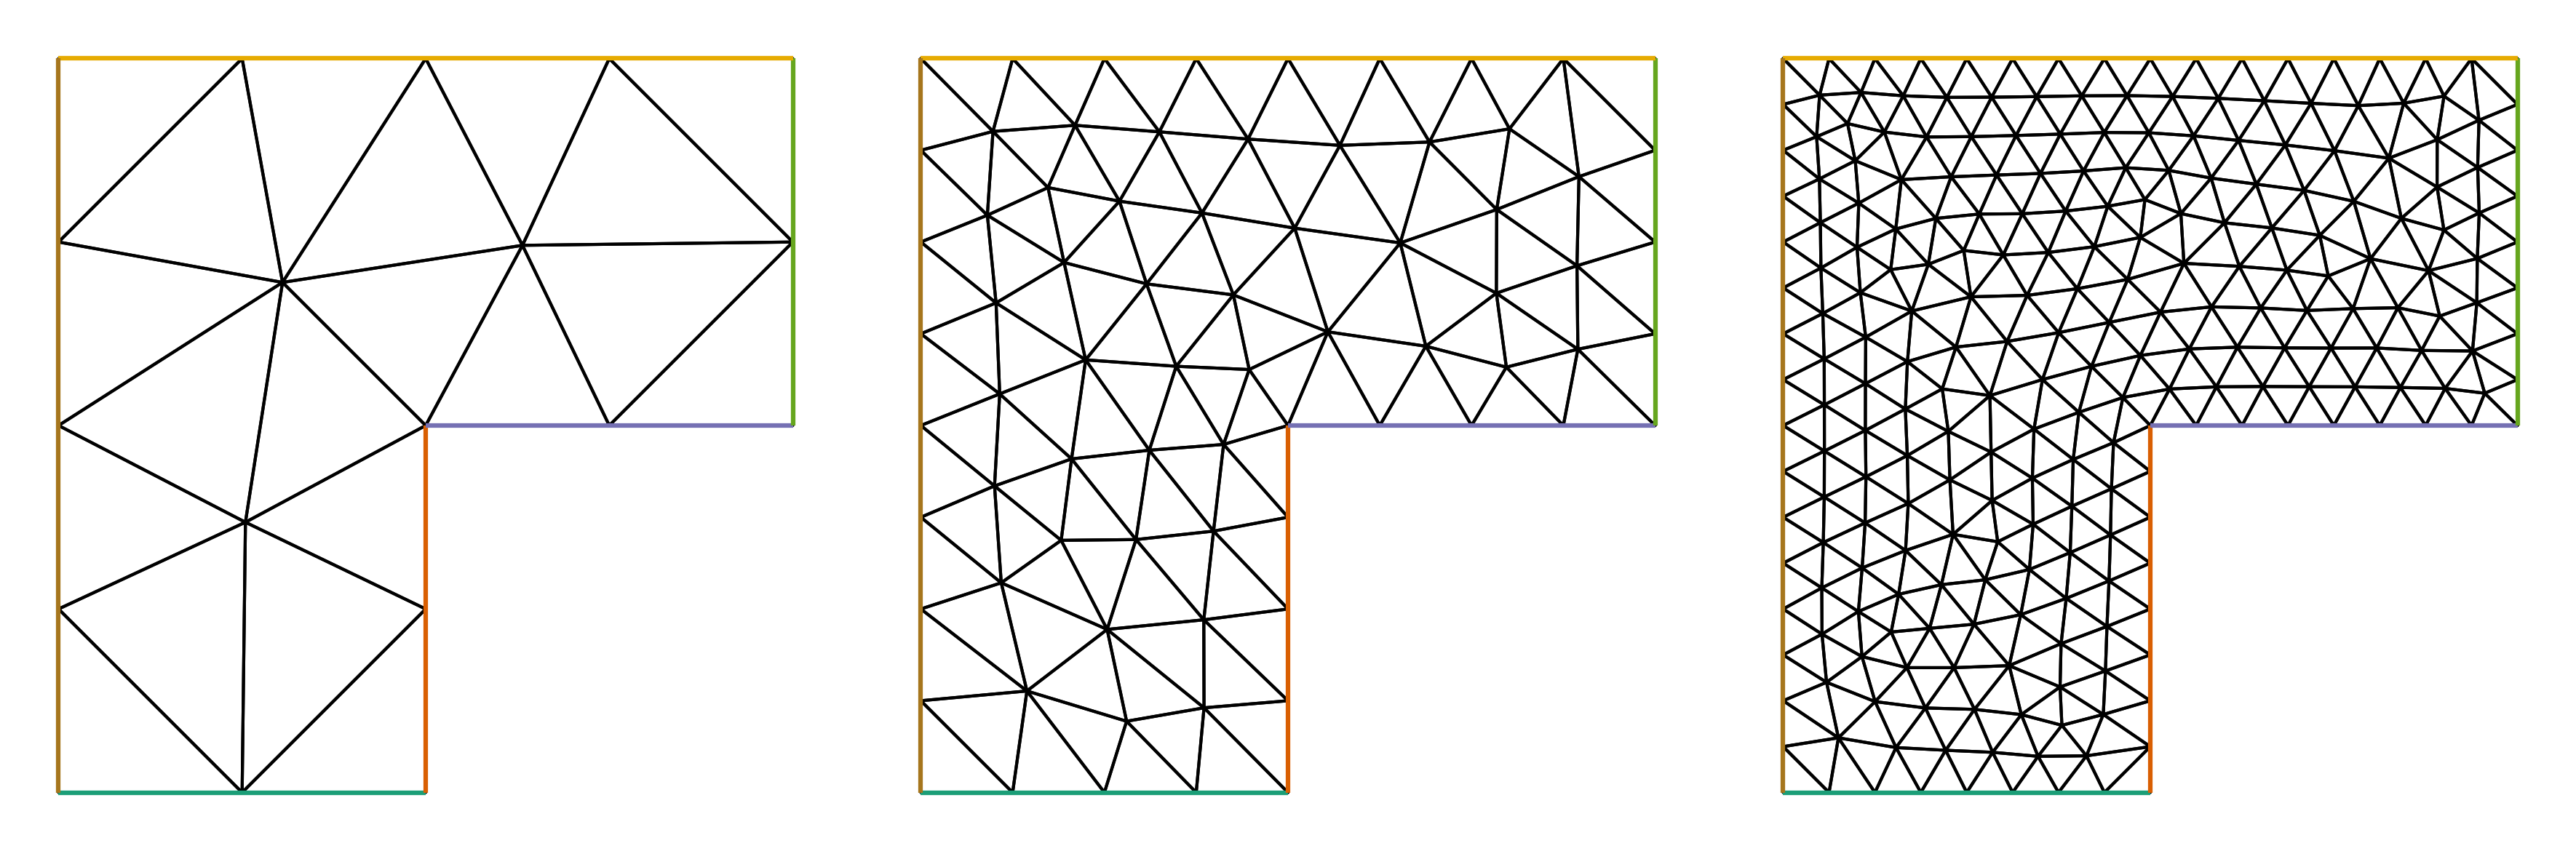
\includegraphics[width=1.0\linewidth]{three_triplots.png}
    \caption{A sequence of unstructured meshes for the desired L-shaped domain ($N = 4, 8, 16$).}
    \label{Lshape}
\end{figure}

\begin{table}[ht]
\centering
\begin{tabular}{c|ccccc}
\toprule
\multicolumn{1}{c}{Exact}
&
\multicolumn{5}{c}{Computed (rate)}
\\
\cmidrule(lr){2-6}
&
$N=4$
&
$N=8$
&
$N=16$
&
$N=32$
&
$N=64$
\\
\midrule
$0.000000$
&
$-0.0000$
&
$0.0000$
&
$-0.0000$
&
$-0.0000$
&
$0.0000$
\\
$1.475622$
&
$1.6722$
&
$1.5263\ (2.0)$
&
$1.4941\ (1.5)$
&
$1.4825\ (1.4)$
&
$1.4782\ (1.4)$
\\
$3.534031$
&
$3.8370$
&
$3.5807\ (2.7)$
&
$3.5462\ (1.9)$
&
$3.5371\ (2.0)$
&
$3.5348\ (2.0)$
\\
$9.869604$
&
$12.0468$
&
$10.2572\ (2.5)$
&
$9.9708\ (1.9)$
&
$9.8937\ (2.1)$
&
$9.8757\ (2.0)$
\\
$9.869604$
&
$12.0985$
&
$10.2835\ (2.4)$
&
$9.9736\ (2.0)$
&
$9.8947\ (2.0)$
&
$9.8758\ (2.0)$
\\
$11.389479$
&
$14.5367$
&
$11.9605\ (2.5)$
&
$11.5314\ (2.0)$
&
$11.4224\ (2.1)$
&
$11.3976\ (2.0)$
\\
\midrule
DOF
&
$19$
&
$74$
&
$248$
&
$936$
&
$3621$
\\
\bottomrule
\end{tabular}
\caption{Computed eigenvalues and observed convergence rates on a sequence of unstructured meshes on the $L$-shaped domain.}
\label{Lshaped_table}
\end{table}


In the presence of singularities, we expect (and observe) lower convergence rates \cite{boffi}. This is apparent in the first nonzero eigenvalue reported in Table \ref{Lshaped_table}, which is associated to an eigenspace of singular eigenfunctions. However, the other eigenvalues are associated to eigenspaces of smooth functions (since the domain is symmetric), and their convergence rate is approximately quadratic\footnote{I do not fully understand this observation.} \cite{boffi}. To emphasize that the convergence rate of the eigenvalues is related to the smoothness of the corresponding eigenfunction, we consider non-adapted meshes. However, in practice, we can improve the convergence by adding more degrees of freedom where they are needed, i.e, in the problematic corner of the L-shaped domain \cite{boffi}.

\subsection{Nonconforming Elements}


Our final experiment for the Lagrange eigenvalue problem is with nonconforming elements.
Recall that a finite element approximation is called conforming if the discrete space, $V_h,$ is a subspace of the infinite-dimensional space, $V,$ in which the variational problem is posed. If $V_h \not\subset V,$ then the approximation is non-conforming.

To explore the impact of nonconforming elements, we consider a sequence of unstructured meshes on the square domain $\Omega = (0, \pi)^2.$ Instead of standard piecewise linear Lagrange finite elements, we will use linear non-conforming triangular elements, known as Crouzeix-Raviart elements \cite{boffi}. The results of this simulation are given in Table \ref{noncon}.

\begin{table}[ht]
\centering
\begin{tabular}{c|ccccc}
\toprule
\multicolumn{1}{c}{Exact}
&
\multicolumn{5}{c}{Computed (rate)}
\\
\cmidrule(lr){2-6}
&
$N=4$
&
$N=8$
&
$N=16$
&
$N=32$
&
$N=64$
\\
\midrule
$2$
&
$1.9686$
&
$1.9899\ (1.6)$
&
$1.9970\ (1.7)$
&
$1.9992\ (2.0)$
&
$1.9998\ (2.0)$
\\
$5$
&
$4.5845$
&
$4.8910\ (1.9)$
&
$4.9730\ (2.0)$
&
$4.9931\ (2.0)$
&
$4.9983\ (2.0)$
\\
$5$
&
$4.6170$
&
$4.9026\ (2.0)$
&
$4.9732\ (1.9)$
&
$4.9933\ (2.0)$
&
$4.9983\ (2.0)$
\\
$8$
&
$7.2805$
&
$7.8294\ (2.1)$
&
$7.9521\ (1.8)$
&
$7.9877\ (2.0)$
&
$7.9968\ (1.9)$
\\
$10$
&
$7.5094$
&
$9.4084\ (2.1)$
&
$9.8670\ (2.2)$
&
$9.9662\ (2.0)$
&
$9.9917\ (2.0)$
\\
$10$
&
$7.9372$
&
$9.4526\ (1.9)$
&
$9.8699\ (2.1)$
&
$9.9668\ (2.0)$
&
$9.9917\ (2.0)$
\\
$13$
&
$9.2454$
&
$12.3977\ (2.6)$
&
$12.8439\ (1.9)$
&
$12.9618\ (2.0)$
&
$12.9902\ (2.0)$
\\
$13$
&
$9.8048$
&
$12.4424\ (2.5)$
&
$12.8565\ (2.0)$
&
$12.9626\ (1.9)$
&
$12.9904\ (2.0)$
\\
$17$
&
$10.7888$
&
$15.2006\ (1.8)$
&
$16.5739\ (2.1)$
&
$16.8914\ (2.0)$
&
$16.9736\ (2.0)$
\\
\midrule
DOF
&
$40$
&
$176$
&
$736$
&
$3008$
&
$12160$
\\
\bottomrule
\end{tabular}
\caption{Computed eigenvalues and observed convergence rates for nonconforming elements on a sequence of unstructured meshes.}
\label{noncon}
\end{table}

As before, we obtain the optimal quadratic rate of convergence in the eigenvalue computations. However, now the computed eigenvalues are lower bounds on the exact eigenvalues. This is typical behaviour for non-conforming approximations and has been reported by several authors \cite{boffi}. In general, conforming approximations of eigenvalues are always above the exact solutions, while nonconforming ones may be below\footnote{In Patrick's Oxford slides, he says that a conforming discretization of a symmetric coercive problem approximates the eigenvalues from above, while a nonconforming discretization, on a sufficiently fine mesh, approximates the eigenvalues from below.}.
For mixed finite element approximations, the situation is more subtle. In some cases, a single discretization may yield upper bounds for some eigenvalues and lower bounds for others \cite{boffi}.

\section{Maxwell Eigenvalue Problem}

We begin with a three-dimensional domain, $\Omega \in \mathbb{R}^3.$ The Maxwell eigenproblem consists of finding the resonant frequencies, $\omega \in \mathbb{R} \setminus \{0\},$ and the electromagnetic fields, $(\mathbf{E}, \mathbf{H}) \ne (\mathbf{0}, \mathbf{0}) \in H_0(\text{curl} ; \Omega) \times H(\text{curl}; \Omega), $ such that
\begin{equation}
\begin{aligned}
\nabla \times \mathbf{E} &= i \, \omega \,  \mu \, \textbf{H}
&& \text{in } \Omega, \\
\nabla \times \textbf{H} &= -i \, \omega \, \varepsilon \, \textbf{E}
&& \text{in } \Omega, \\
\textbf{E} \times \textbf{n} &= 0
&& \text{on } \partial\Omega .
\end{aligned}
\end{equation}
Here, $H(\text{curl}; \Omega)$ is the space of vector fields in $(L^2(\Omega))^3$ with curl in $(L^2(\Omega))^3$ and $H_0(\text{curl}; \Omega)$ is the space of elements of $H(\text{curl}; \Omega)$ that have vanishing tangential trace on $\partial \Omega.$ Furthermore, $\textbf{n}$ is the outward normal for $\partial \Omega,$ while
$\varepsilon$ and $\mu$ are the dielectric permitivity and magnetic permeability, respectively \cite{boffi}. We will assume that both $\varepsilon$ and $\mu$ are equal to the identity matrix. In doing so, we eliminate $\mathbf{H}$ and obtain the more common formulation of the problem: find $\omega \in \mathbb{R} \setminus \{0\}$ and $\mathbf{u} \ne \mathbf{0} \in H_0(\text{curl}; \Omega),$ such that
\begin{equation}
\begin{aligned}
    \nabla \times \nabla \times \mathbf{u}
 &=
\omega^2 \, \mathbf{u}  
\qquad \text{in } \Omega, \\
\mathbf{u}\times \textbf{n} &= 0
\qquad \text{on } \partial\Omega .
\end{aligned}
\end{equation}

To construct the variational formulation, we take the inner product with a $v \in H_0(\text{curl}; \Omega)$ and integrate by parts\footnote{Using the integration by parts identity for the $\text{curl},$ i.e., $\int_{\Omega} \text{curl}\mathbf{A} \cdot \overline{\mathbf{v}} \, d\textbf{x} = \int_{\Omega} \mathbf{A} \cdot \text{curl} \overline{\mathbf{v}} \, d\textbf{x} + \int_{\partial \Omega} (\mathbf{n} \times \mathbf{A}) \cdot \overline{\mathbf{v}} \, d\textbf{s},$ with $\mathbf{A} = \text{curl}\mathbf{E}.$ } to obtain: find $\omega \in \mathbb{R}\setminus \{0\}$ and $u \ne 0 \in H_0(\text{curl}; \Omega)$ such that
\begin{equation}
    \int_{\Omega} \text{curl}\mathbf{u} \cdot \text{curl}\overline{\mathbf{v}} \, dx = \omega^2 \int_{\Omega} \mathbf{u} \cdot \overline{\mathbf{v}} \, dx,
\end{equation}
for all $v \in H_0(\text{curl}; \Omega).$

Notice that if $\omega = 0,$ the problem reduces to finding the nullspace of the curl operator \cite{Matt}. This is an infinite-dimensional space, since it contains the gradients of all smooth functions that vanish on the boundary of $\Omega$ \cite{Arnold}.  Thus, a bad finite element space may produce approximations, $u_h,$ that look almost like zero-curl modes, i.e., $\text{curl} \mathbf{u}_h \approx 0,$ but are not true physical modes. Numerically, this creates fake computed eigenvalues \cite{Matt}. A good choice of finite element space will respect the following decomposition of $H_0(\text{curl}; \Omega),$
\begin{equation}
    H_0(\text{curl}; \Omega) = N(\text{curl}) \oplus (\text{physical} \, \mathbf{u}_h).
\end{equation}
We will further explore this potential for \textit{spectral pollution }in the two-dimensional case. 

In two dimensions, we consider $\Omega = (0, \pi)^2$ and seek $\omega \in \mathbb{R} \setminus \{0\}$ and nonzero $(\mathbf{E}, H) \in H_0(\text{rot}; \Omega) \times H(\text{\textbf{rot}}; \Omega)$ such that 
\begin{equation}
    \begin{aligned}
\operatorname{rot} \textbf{E} &= i \, \omega \, H
&& \text{in } \Omega,\\
\operatorname{\textbf{rot}} H &= -i\, \omega \,  \textbf{E}
&& \text{in } \Omega,\\
\textbf{E}\cdot \textbf{t} &= 0,
&& \text{on } \partial\Omega,
\end{aligned}
\end{equation}
where 
\begin{equation}
    \operatorname{rot} \mathbf{E}
=
\frac{\partial E_2}{\partial x}
-
\frac{\partial E_1}{\partial y},
\qquad
\operatorname{\textbf{rot}} H
=
\begin{pmatrix}
\frac{\partial H}{\partial y}\\
-\frac{\partial H}{\partial x}
\end{pmatrix},
\end{equation}
and $\mathbf{t}$ is the unit tangent to $\partial \Omega.$ Here, $H_0(\text{rot}; \Omega)$ is the space of functions in $(L^2(\Omega))^2$ who have vanishing tangential trace on $\partial \Omega$ and whose $\text{rot}$ is in $L^2(\Omega).$ Similarly, $H(\text{\textbf{rot}}; \Omega)$ is the space of functions in $L^2(\Omega)$ with $\text{\textbf{rot}}$ in $(L^2(\Omega))^2.$ 

Solving for $H,$ taking the inner product with a $v \in H_0(\text{rot}; \Omega),$ and integrating by parts, we obtain the variational formulation: find $\omega \in \mathbb{R}\setminus \{0\}$ and $\mathbf{u} \ne 0 \in H_0(\text{rot}; \Omega)$ such that
\begin{equation}
    \int_{\Omega} \text{rot} \, \textbf{u} \,\, \overline{\text{rot} \, \textbf{v}} \, d\mathbf{x} = \omega^2 \int_{\Omega} \textbf{u} \cdot \overline{\textbf{v}} \, d\textbf{x},
\end{equation}
for all $\mathbf{v} \in H_0(\text{rot}; \Omega).$
To discretize the problem, we restrict ourselves to a finite-dimensional space, $V_h,$ and seek 
$\omega \in \mathbb{R}\setminus \{0\}$ and $\mathbf{u}_h \ne 0 \in V_h$ such that
\begin{equation}
    \int_{\Omega} \text{rot} \, \textbf{u}_h \,\, \overline{\text{rot} \, \textbf{v}} \, d\mathbf{x} = \omega^2 \int_{\Omega} \textbf{u}_h \cdot \overline{\textbf{v}} \, d\textbf{x},
\end{equation}
for all $\mathbf{v} \in V_h.$

This problem shares the spectral pollution dangers of its three-dimensional counterpart \cite{Matt}. Furthermore, the squares of the eigenvalues, $\omega^2,$ correspond to the Neumann eigenvalues of the Laplacian in $\Omega,$ i.e.,
\begin{equation}
    w^2 = n^2 + m^2,
\end{equation}
for $m, n \in \mathbb{N}_0$ and $(m, n) \ne (0, 0)$ \cite{boffi}. This property makes this version of the Maxwell eigenproblem a famous example for exploring the effects of spectral pollution and for validating methods for computing spectra.

To see the effects of spectral pollution, we first consider piecewise linear finite elements on a sequence of structured meshes. The results on a sequence of structured meshes are displayed in Figure \ref{maxwellCG1}. Notice that the zero frequency is not well approximated, and it seems that bad approximations of
the zero frequency pollute the whole spectrum \cite{boffi}. Indeed, it can be observed that the correct values are well approximated together
with their eigenfunctions, but their approximations are hardly distinguishable from spurious solutions \cite{boffiB}. Keeping this in mind, we may expect that it is enough to choose a finite element space that represents gradient fields well, so that the zero-freqeuncy modes are accurately approximated. However, this is not sufficient to eliminate spectral pollution \cite{boffi}. For example, even if we choose piecewise linear elements on a sequence of criss-cross meshes, where gradients are well represented, we obtain spurious eigenvalues. This result is illustrated by Table \ref{spect pollute}. 


\begin{figure}[ht]
\centering

\begin{subfigure}[t]{0.31\textwidth}
    \centering
    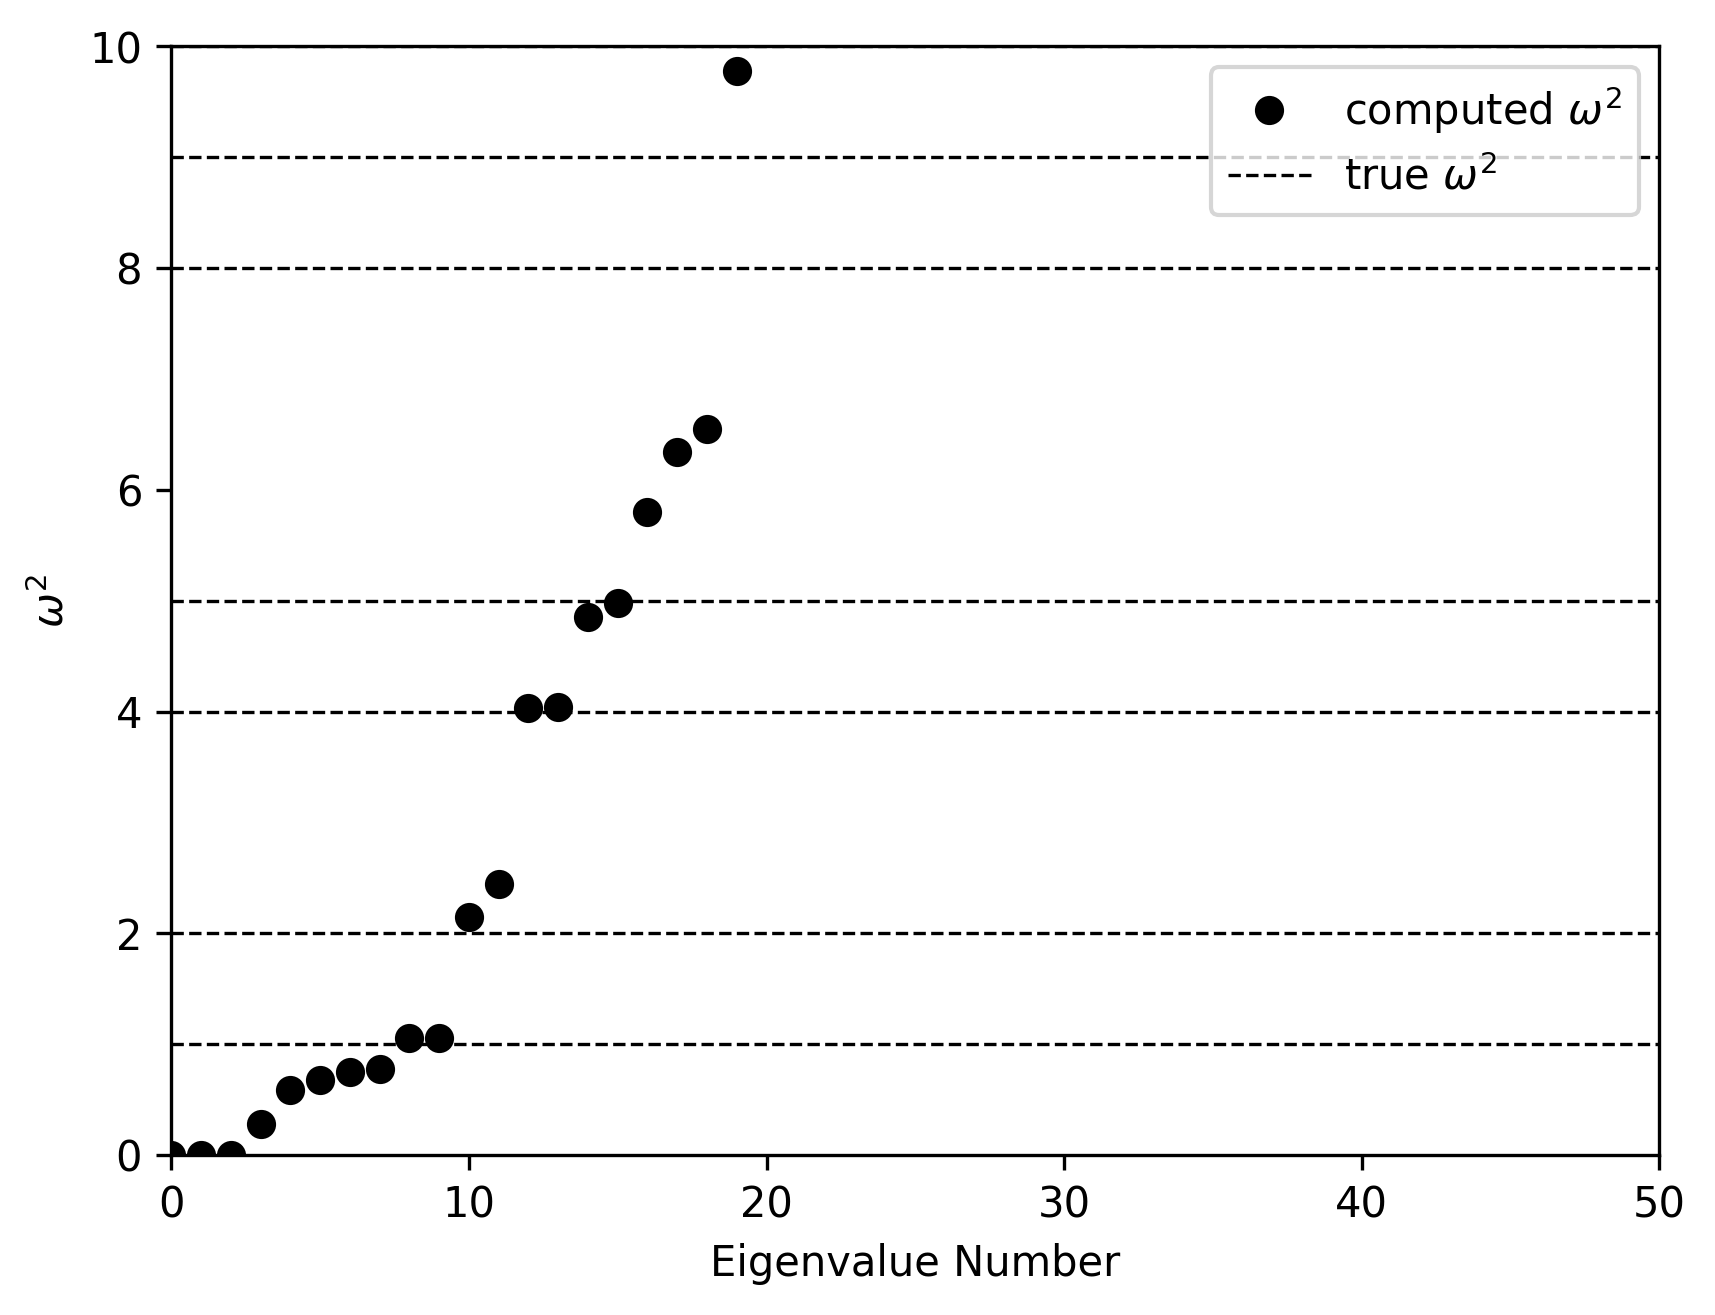
\includegraphics[width=\textwidth]{Maxwell_CG1_N4 (3).png}
    \caption{$N=4$}
    \label{fig:maxwell-N4}
\end{subfigure}
\hfill
\begin{subfigure}[t]{0.31\textwidth}
    \centering
    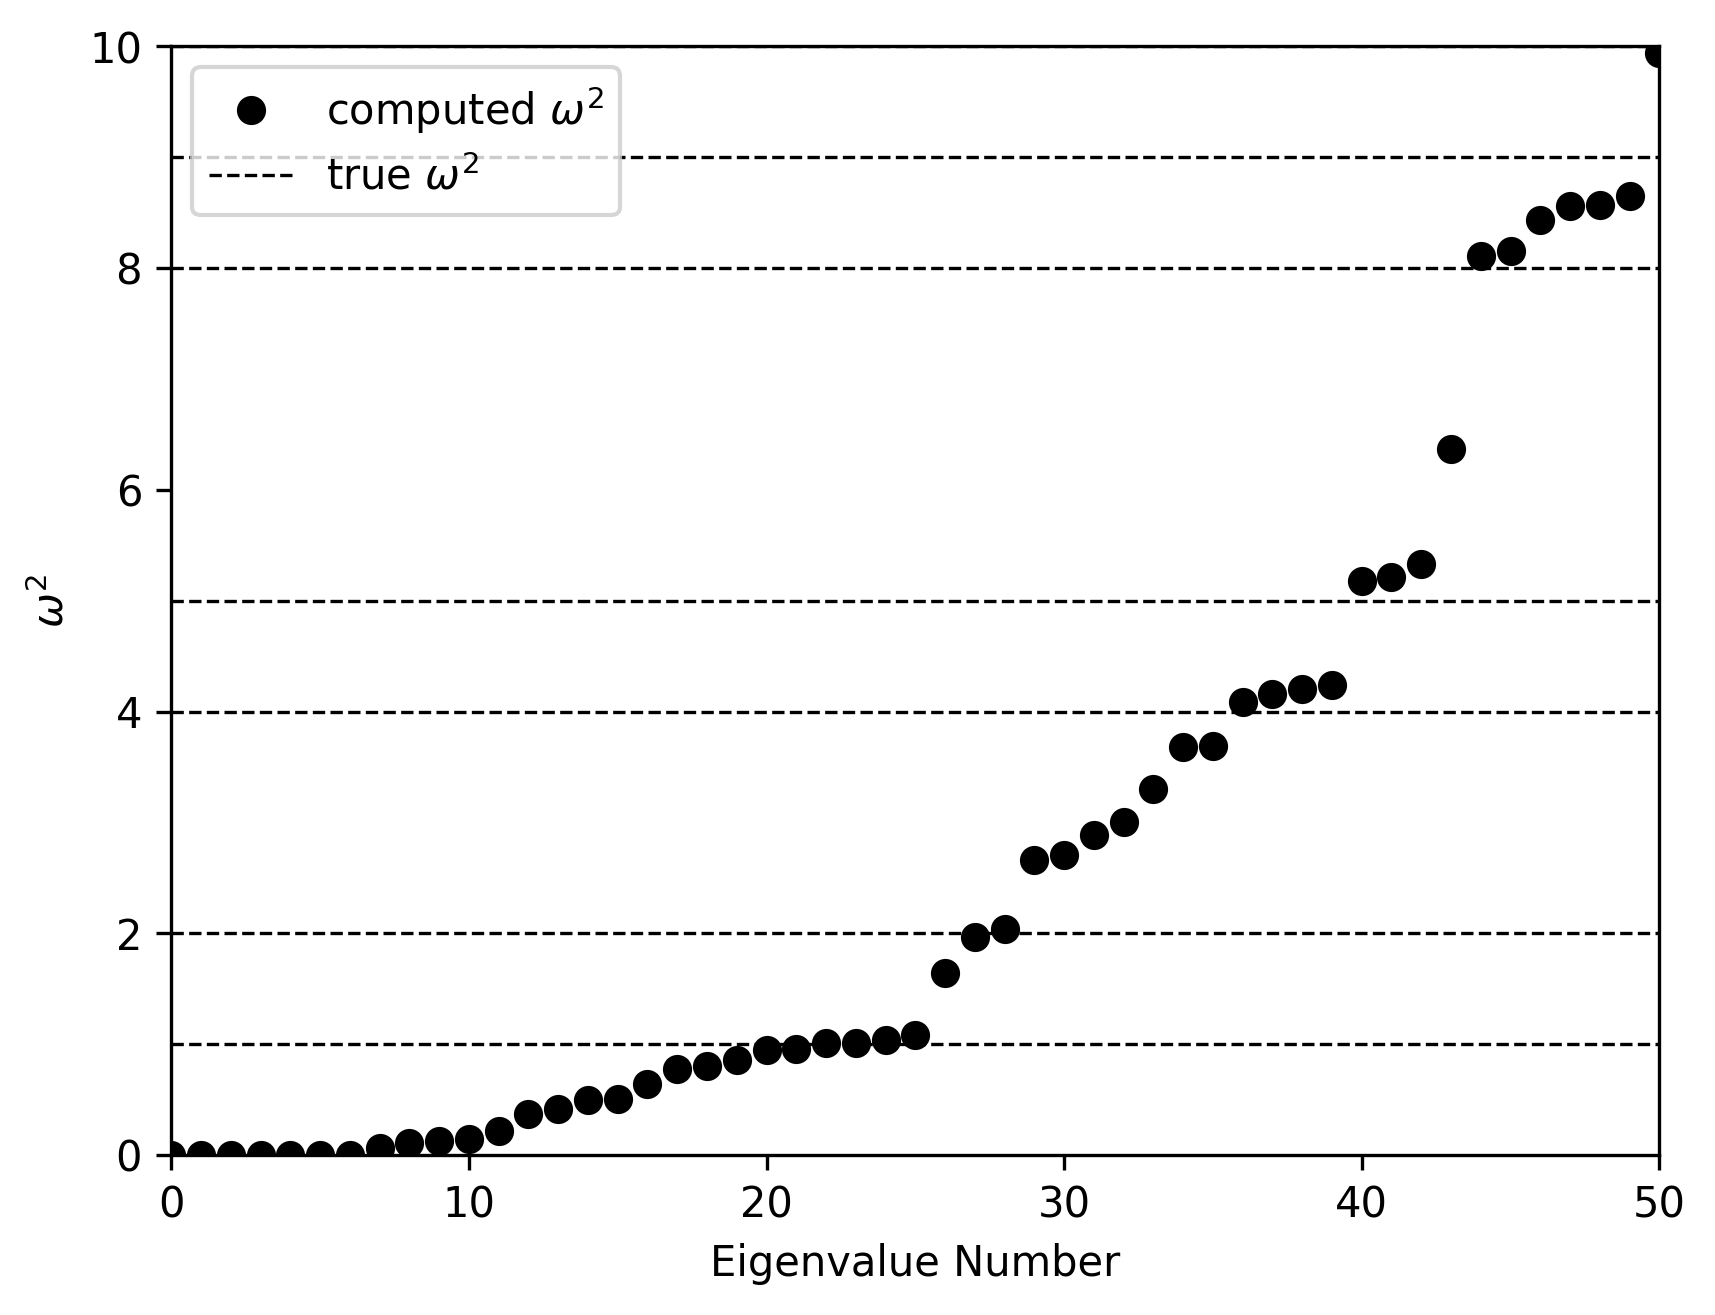
\includegraphics[width=\textwidth]{Maxwell_CG1_N8 (3).png}
    \caption{$N=8$}
    \label{fig:maxwell-N8}
\end{subfigure}
\hfill
\begin{subfigure}[t]{0.31\textwidth}
    \centering
    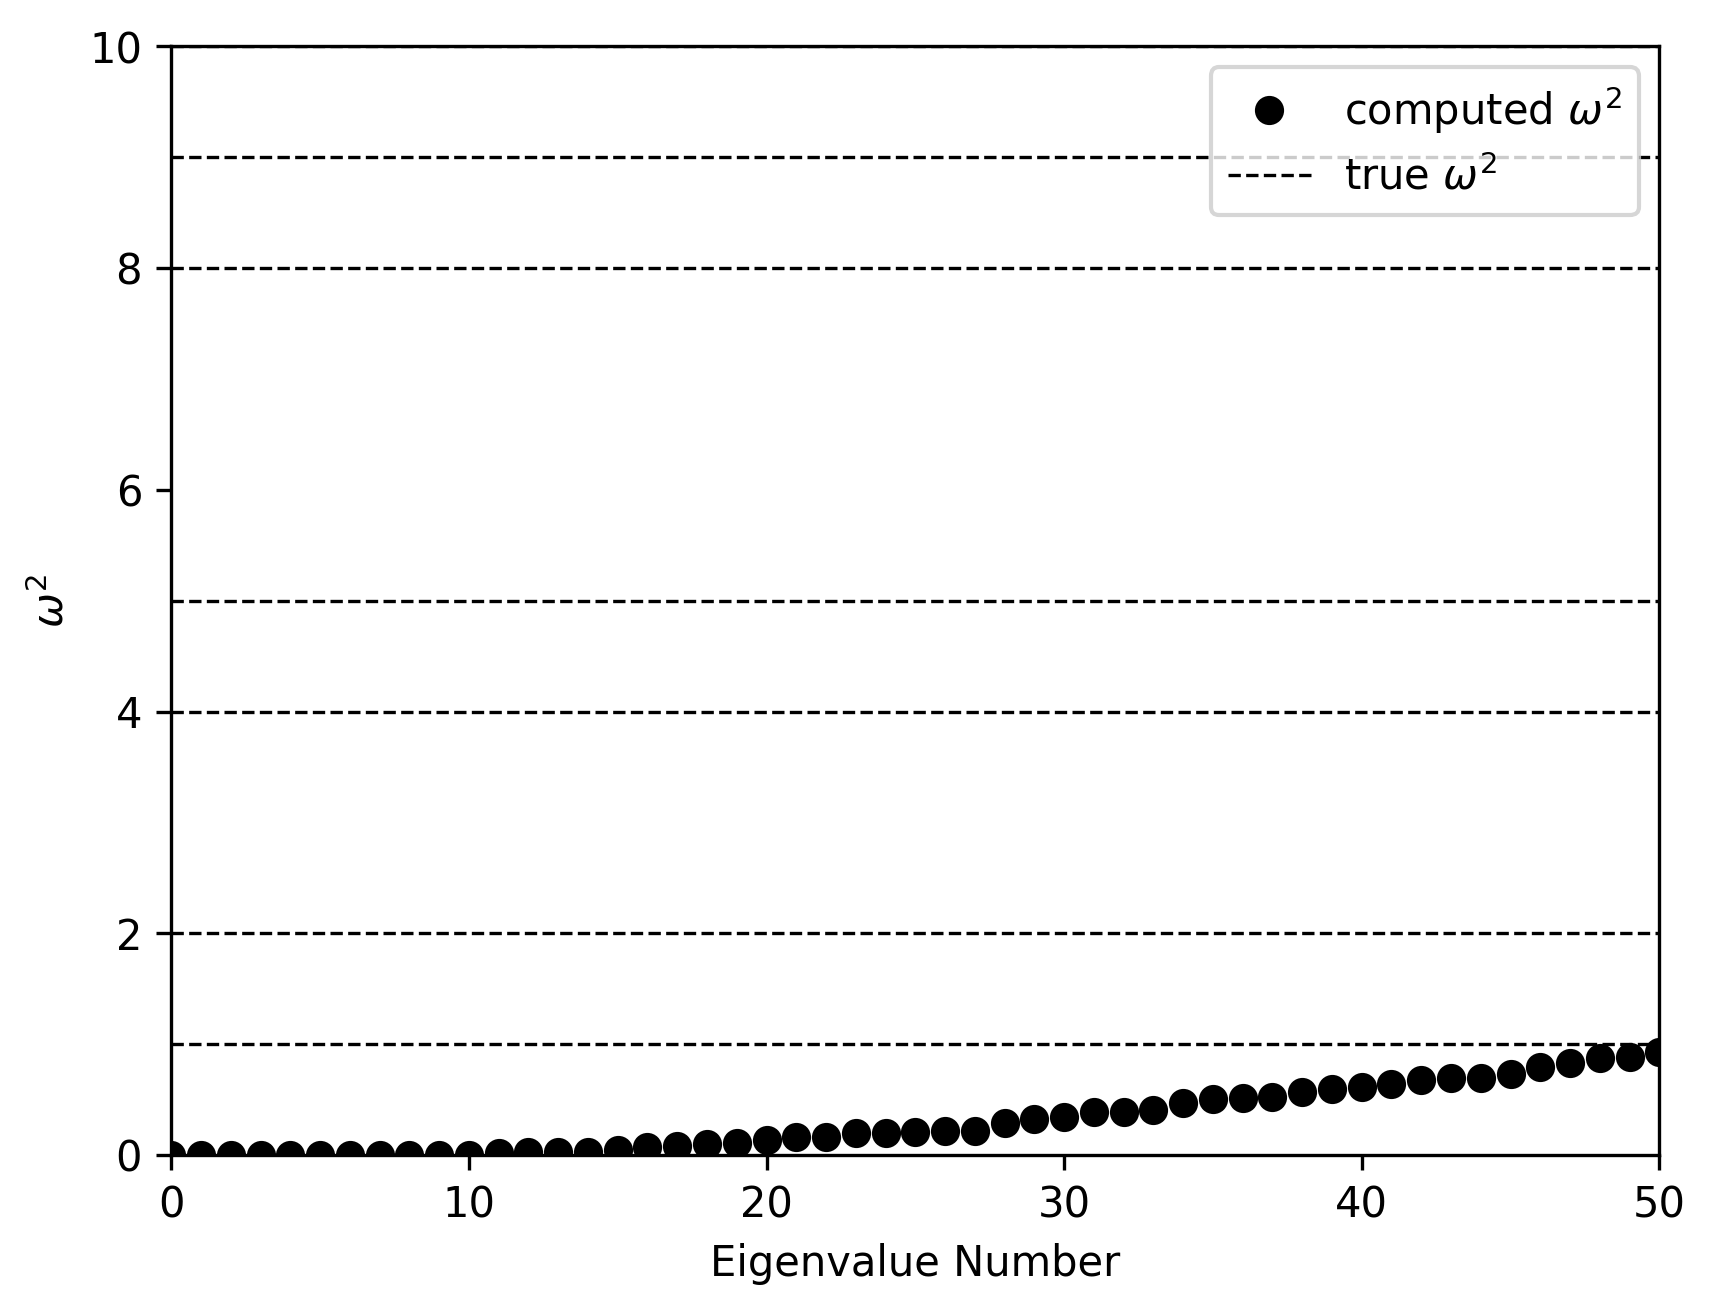
\includegraphics[width=\textwidth]{Maxwell_CG1_N16 (2).png}
    \caption{$N=16$}
    \label{fig:maxwell-N16}
\end{subfigure}

\caption{The first 50 discrete eigenvalues for the Maxwell eigenproblem. These are computed using piecewise linear elements on structured meshes for $N=4,8,16$. We note that the \texttt{SLEPSc} target eigenvalue was set to one for these computations.}
\label{maxwellCG1}
\end{figure}

\begin{table}[ht]
\centering
\begin{tabular}{c|ccccc}
\toprule
\multicolumn{1}{c}{Exact}
&
\multicolumn{5}{c}{Computed (rate)}
\\
\cmidrule(lr){2-6}
&
$N=4$
&
$N=8$
&
$N=16$
&
$N=32$
&
$N=64$
\\
\midrule
$1$
&
$1.0170$
&
$1.0043\ (2.0)$
&
$1.0011\ (2.0)$
&
$1.0003\ (2.0)$
&
$1.0001\ (2.0)$
\\
$1$
&
$1.0170$
&
$1.0043\ (2.0)$
&
$1.0011\ (2.0)$
&
$1.0003\ (2.0)$
&
$1.0001\ (2.0)$
\\
$2$
&
$2.0678$
&
$2.0171\ (2.0)$
&
$2.0043\ (2.0)$
&
$2.0011\ (2.0)$
&
$2.0003\ (2.0)$
\\
$4$
&
$4.2647$
&
$4.0680\ (2.0)$
&
$4.0171\ (2.0)$
&
$4.0043\ (2.0)$
&
$4.0011\ (2.0)$
\\
$4$
&
$4.2647$
&
$4.0680\ (2.0)$
&
$4.0171\ (2.0)$
&
$4.0043\ (2.0)$
&
$4.0011\ (2.0)$
\\
$5$
&
$5.3971$
&
$5.1063\ (1.9)$
&
$5.0267\ (2.0)$
&
$5.0067\ (2.0)$
&
$5.0017\ (2.0)$
\\
$5$
&
$5.3971$
&
$5.1063\ (1.9)$
&
$5.0267\ (2.0)$
&
$5.0067\ (2.0)$
&
$5.0017\ (2.0)$
\\
\textcolor{red}{$6$}
&
\textcolor{red}{$5.6712$}
&
\textcolor{red}{$5.9229\ (2.1)$}
&
\textcolor{red}{$5.9807\ (2.0)$}
&
\textcolor{red}{$5.9952\ (2.0)$}
&
\textcolor{red}{$5.9988\ (2.0)$}
\\
$8$
&
$8.8141$
&
$8.2713\ (1.6)$
&
$8.0685\ (2.0)$
&
$8.0171\ (2.0)$
&
$8.0043\ (2.0)$
\\
$9$
&
$10.2540$
&
$9.3408\ (1.9)$
&
$9.0864\ (2.0)$
&
$9.0217\ (2.0)$
&
$9.0054\ (2.0)$
\\
$9$
&
$10.2540$
&
$9.3408\ (1.9)$
&
$9.0864\ (2.0)$
&
$9.0217\ (2.0)$
&
$9.0054\ (2.0)$
\\
\midrule
DOF
&
$62$
&
$254$
&
$1022$
&
$4094$
&
$16382$
\\
\bottomrule
\end{tabular}
\caption{Computed nonzero eigenvalues and the observed convergence rates for the Maxwell eigenproblem on a sequence of criss-cross meshes. The red row indicates a spurious eigenvalue.}
\label{spect pollute}
\end{table}
% DOF is 4N^2 - 2
% 62, 254, 1022, 4094, 16382


In general, for this example, whether spectral pollution occurs depends on the choice of mesh and finite elements. For example, if we choose (Nédélec) edge elements, there is no spectral pollution. This result is illustrated in Figure \ref{nedelec}. The lack of spectral pollution when using edge elements can be explained using the de Rham complex\footnote{I want to return to this explanation, understand it better, and rewrite it.} \cite{Arnold}. In particular, edge elements allow the normal component of the vector field to jump across element interfaces, while enforcing continuity of the tangential component. This is the correct continuity requirement for the Maxwell eigenproblem. As a result, the discrete gradient fields are represented in the nullspace of the discrete curl operator, so the $\omega = 0$ modes are well approximated.
% since edge elements are $H(\text{curl})$ conforming, they
% hey allow the normal component of the vector field to jump across elements, while keeping the tangential component continuous. This preservation of the de Rham complex allows for the exact representation of the $\omega = 0$ gradient fields (the discrete curl operator has a massive nullspace consisting of the gradients of discrete scalar functions). 
This is not the case for Lagrange elements, which enforce the continuity of the tangential and the normal components of the vector field across elements. This continuity constraint leads the discretization to poorly approximate the nullspace of the curl operator, which can lead to nonphysical spurious results.

\begin{figure}[ht]
\centering

\begin{subfigure}[t]{0.31\textwidth}
    \centering
    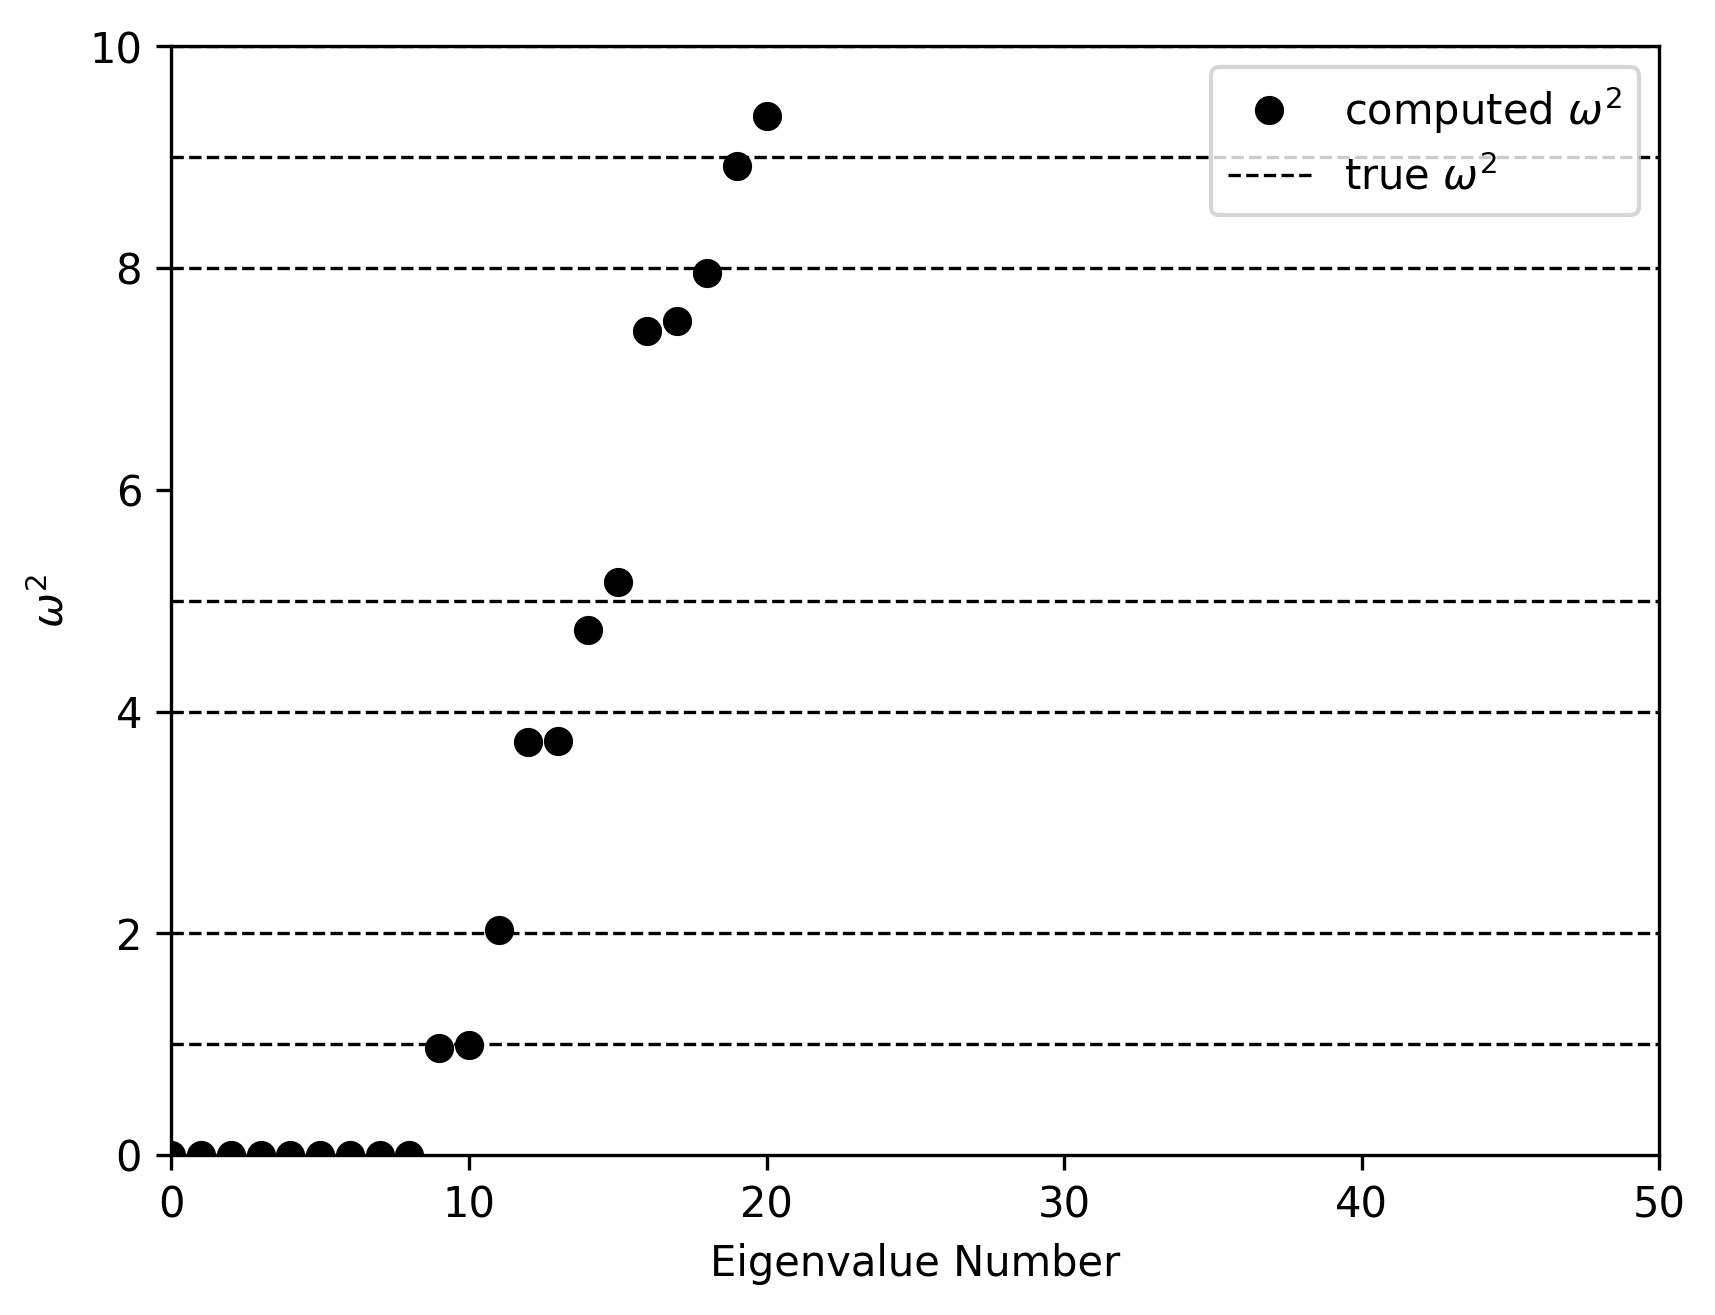
\includegraphics[width=\textwidth]{Maxwell_Nedelec_N4 (1).png}
    \caption{$N=4$}
    % \label{fig:maxwell-N4}
\end{subfigure}
\hfill
\begin{subfigure}[t]{0.31\textwidth}
    \centering
    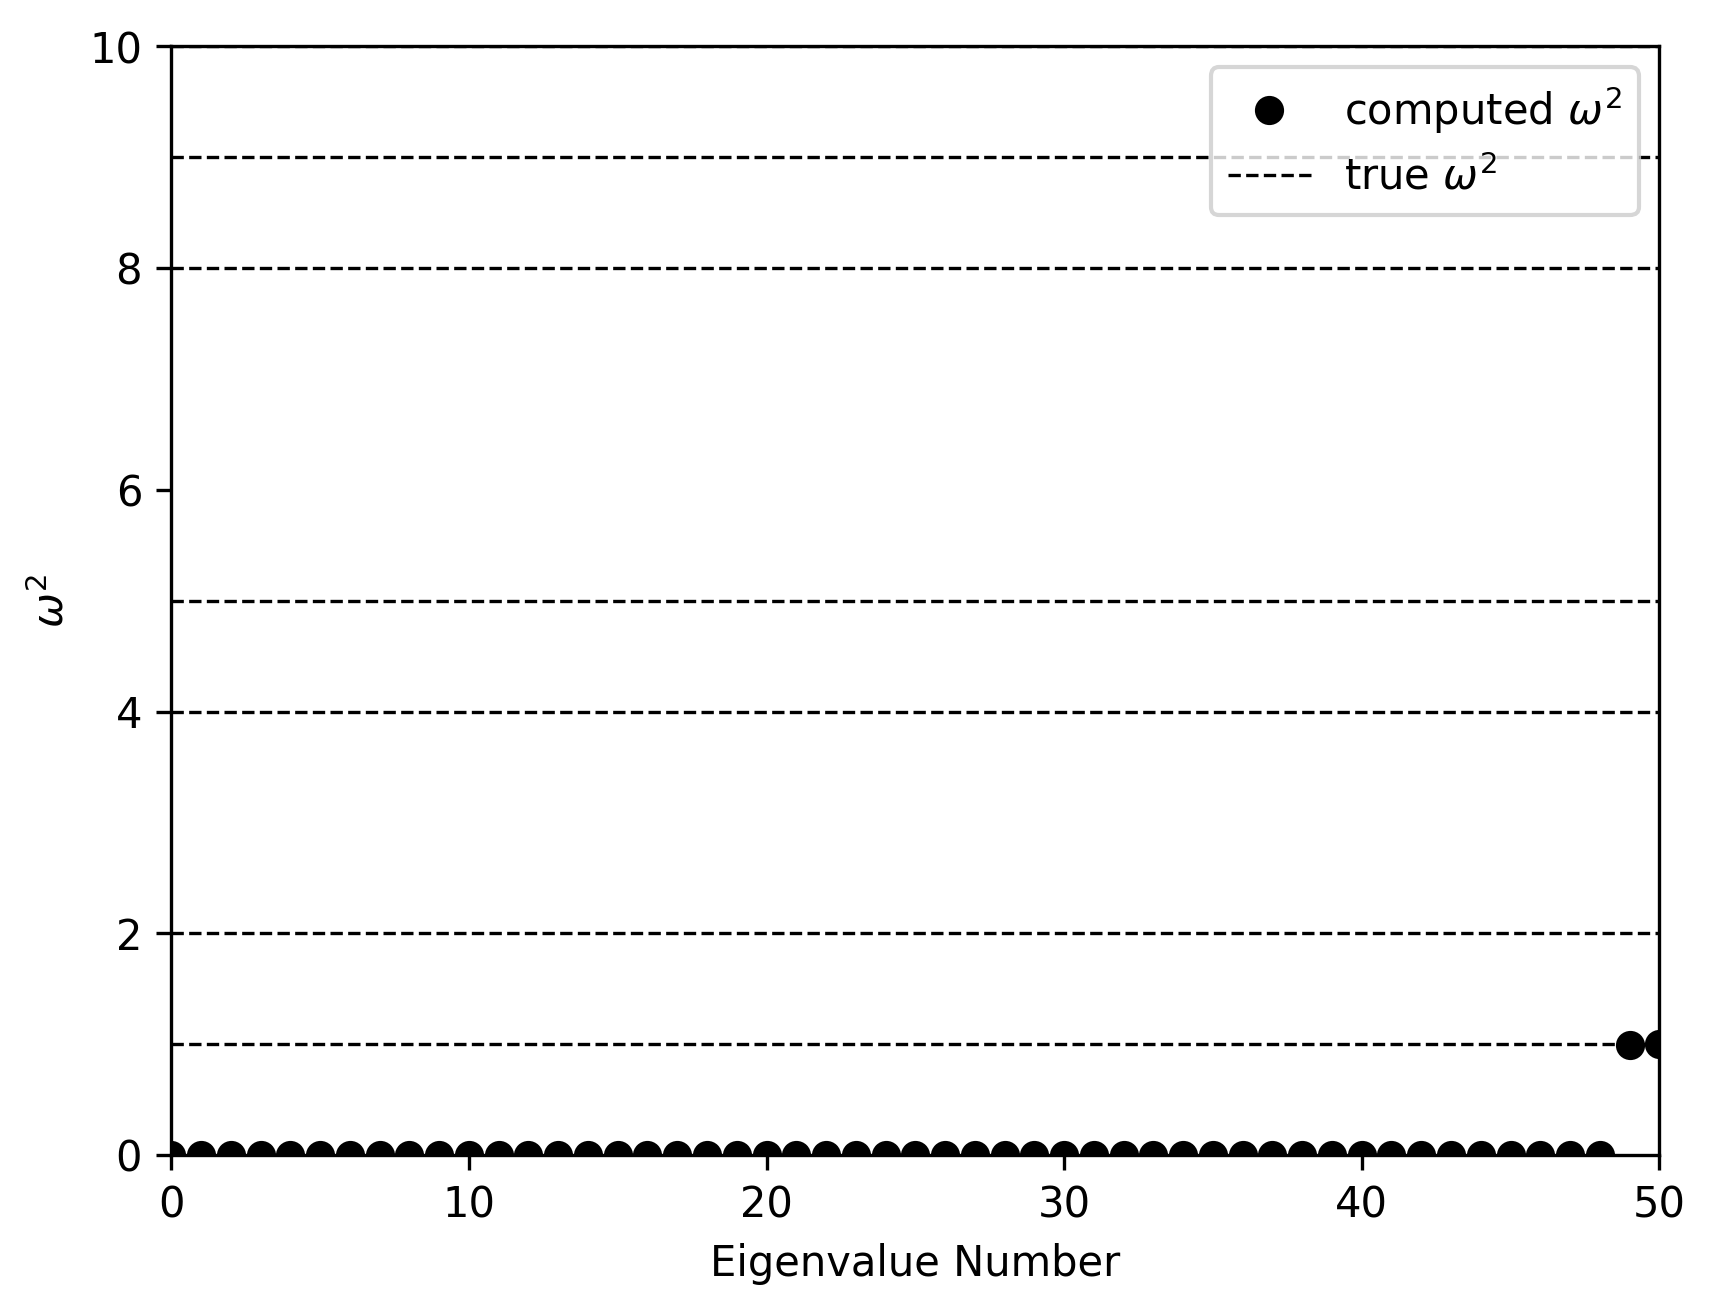
\includegraphics[width=\textwidth]{Maxwell_Nedelec_N8 (1).png}
    \caption{$N=8$}
    % \label{fig:maxwell-N8}
\end{subfigure}
\hfill
\begin{subfigure}[t]{0.31\textwidth}
    \centering
    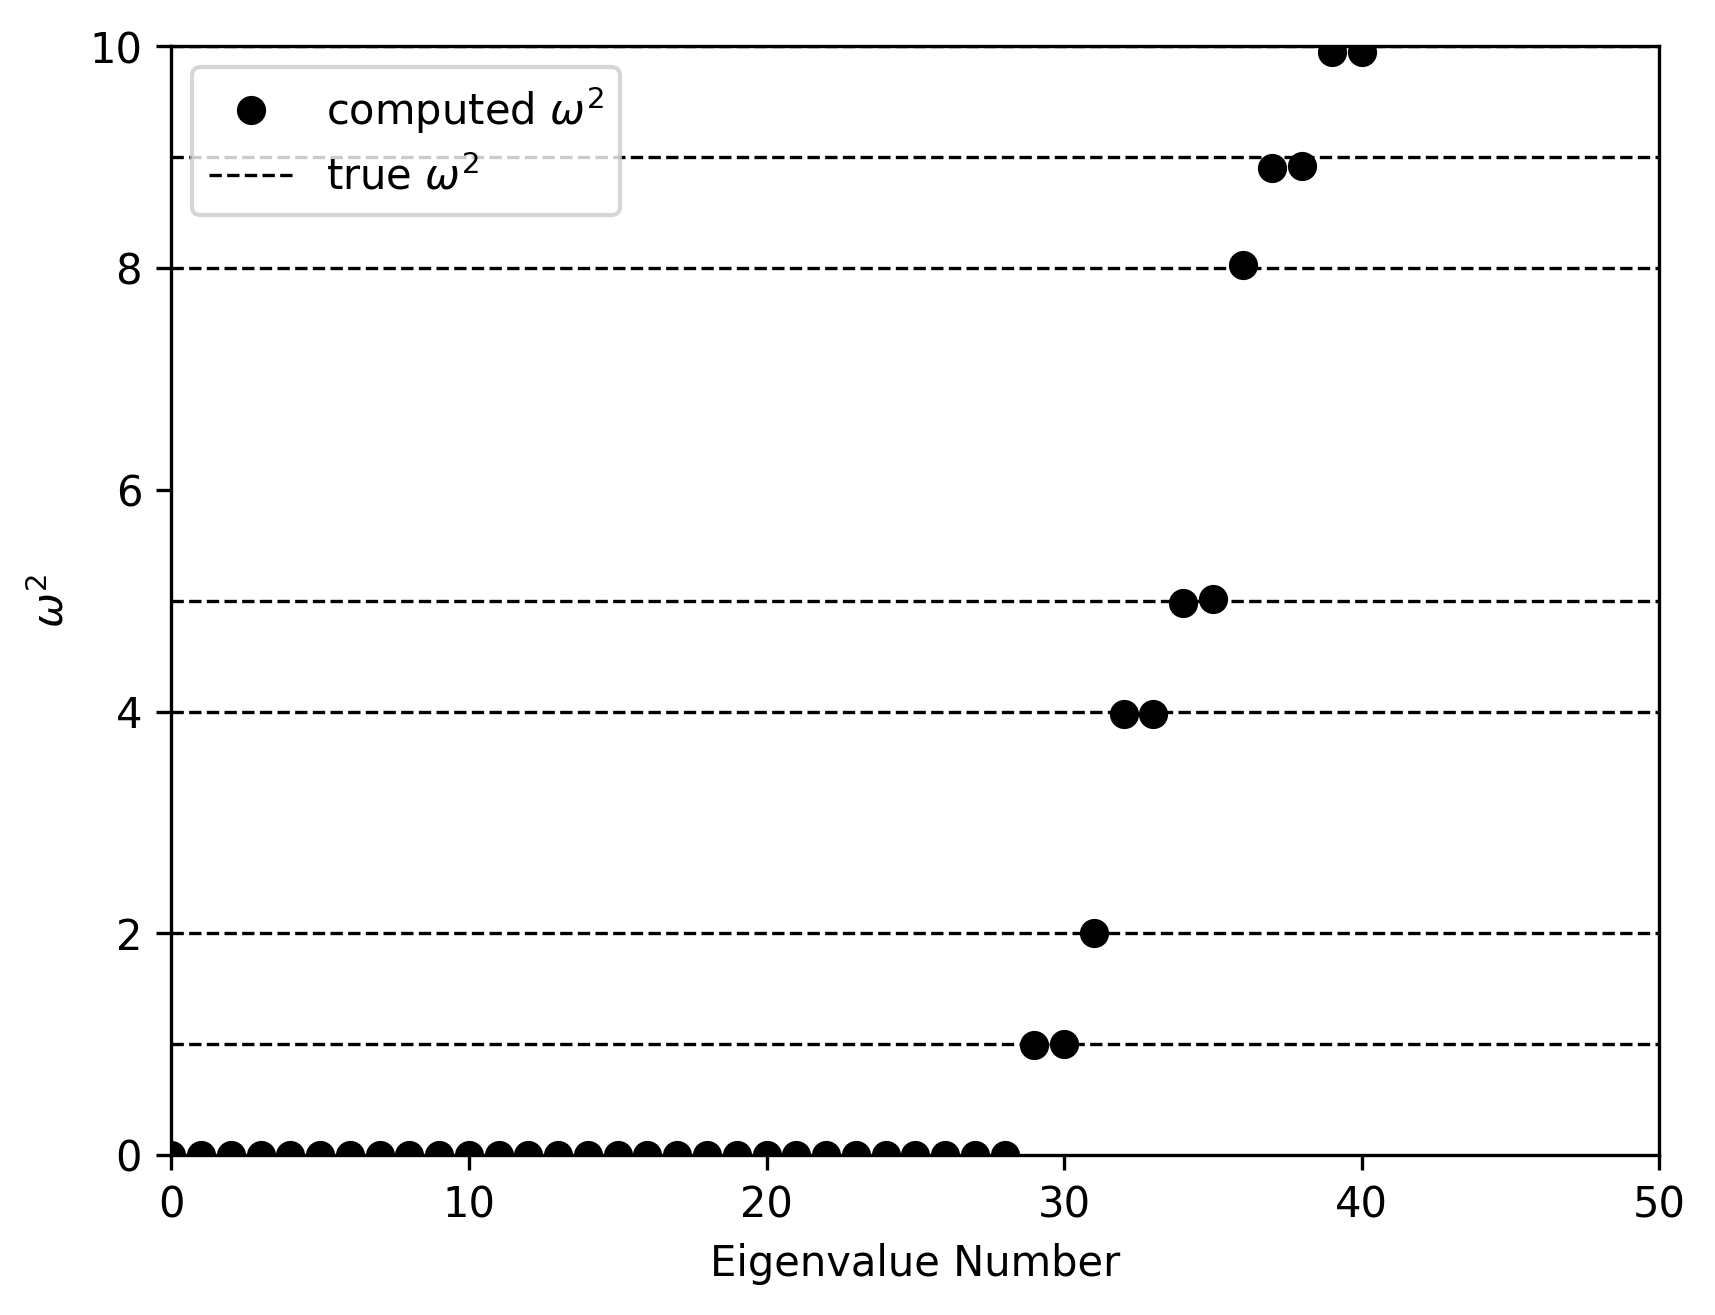
\includegraphics[width=\textwidth]{Maxwell_Nedelec_N16 (1).png}
    \caption{$N=16$}
    % \label{fig:maxwell-N16}
\end{subfigure}

\caption{The first 50 discrete eigenvalues for the Maxwell eigenproblem. These are computed using edge elements on structured meshes for $N=4,8,16$. We note that the \texttt{SLEPSc} target eigenvalue was set to one for these computations.}
\label{nedelec}
\end{figure}



\section{Some Brief Notes on Boffi Part Two}

\subsection{Symmetric Problems, Compact Operators}

\textbf{Beginner definitions:}

\begin{itemize}
    \item $X$ is a complex Hilbert space and $T:X \rightarrow X$ is a compact linear operator.
    \item The resolvent set, $\rho(T),$ is the set of $z \in \mathbb{C}$ such that $(zI - T),$ denoted $(z-T),$ is bijective. The resolvent operator is $(z - T)^{-1}.$ The spectrum, $\sigma(T),$ is the complement of the resolvent set. 
    \item The ascent multiplicity is the smallest integer such that $\text{ker}(\lambda - T)^{\alpha} = \text{ker}(\lambda - T)^{\alpha + 1},$ where $\lambda$ is a nonvanishing eigenvalue of $T.$ The descent multiplicity is defined analagously, using the range instead of the kernel.
    \item The algebraic multiplicity of $\lambda$ is the dimension of $\text{ker}(\lambda - T)^{\alpha}.$
    \item The geometric multiplicity is the dimension of $\text{ker}(\lambda - T).$
    \item The elements of $\text{ker}(\lambda - T)^{\alpha}$ are the generalized eigenvectors of $T$ associated with $\lambda.$ A generalized eigenvector is of order $k$ if it is an element of $\text{ker}(\lambda - T)^{k}$ but not $\text{ker}(\lambda - T)^{k}.$
\end{itemize}

\textbf{Properties of Compact $T$:}

\begin{itemize}
    \item The spectrum of a compact operator is a countable set with no limit points different from zero. 
    \item When $T$ is compact, all nonzero spectral values are eigenvalues.
    \item When $T$ is compact, its ascent and descent multiplicities coincide.
\end{itemize}

\textbf{The adjoint:}
\begin{itemize}
    \item $\lambda \in \sigma(T^*)$ $\iff$ $\overline \lambda \in \sigma(T).$
    \item The eigenvalues of self adjoint operators are real. 
    \item The algebraic multiplicity of $\lambda \in \sigma(T^*)$ equals the algebraic multiplicity of $\overline \lambda \in \sigma(T).$ The ascent multiplicity of $\lambda - T^*$ is equal to that of $\overline \lambda - T.$
\end{itemize}

\textbf{The Riesz Spectral Projection:}

\begin{itemize}
    \item Let $\Gamma \subset \rho(T)$ be a closed smooth curve that defined a single spectral point, $\lambda \in \sigma(T).$ The Riesz spectral projection associated with $\lambda$ is 
    $$ E(\lambda) = \frac{1}{2 \pi i} \int_{\Gamma} (z-T)^{-1} \, dz.$$
    This definition does not depend on the choice of $\Gamma.$
    \item We note that $E(\lambda):X \rightarrow X,$ and $$E(\lambda)(X) = \text{ker}(\lambda - T)^{\alpha}.$$
    \item In general, if $\Gamma \subset \rho(T)$ encloses more spectral points, then 
    $$ E(\lambda_1, \dots, \lambda_n) X = \oplus_{i=1}^{n} \text{ker}(\lambda_i - T)^{\alpha_i}.$$
\end{itemize}


\textbf{Variational eigenproblems:}

\begin{itemize}
    \item Let $V$ and $H$ be real Hilbert spaces, where $V \subset H$ with a dense continuous embedding. Let $a: V \times V \rightarrow \mathbb{R}$ and $b:H\times H \rightarrow \mathbb{R}$ be continuous and symmetric bilinear forms. We want to find $\lambda \in \mathbb{R}$ and a nonzero $u\in V$ such that 
    $$a(u, v) = \lambda b(u, v)\qquad \forall v \in V.$$
    \item We further assume that $a$ is $v$-elliptic and that $b$ is a scalar product in $H.$

    \item Consider a compact $T:H\rightarrow H.$ Given an $f \in H,$ there exists a unique $Tf \in V$ such that 
    $$a(Tf, v) = b(f, v) \qquad \forall v \in V.$$

    \item Since $a$ and $b$ are symmetric, $T$ is also self-adjoint. Thus, $\sigma(T)$ is a countable set  or is a finite set of real numbers with a cluster point possible only at zero. All positve elements of $\sigma(T)$ are eigenvalues with finite multiplicity and their reciprocals are exactly the eigenvalues of $a(u, v) = \lambda b(u, v).$ Furthermore, the eigensolutions of $a(u,v)=\lambda b(u,v)$ have the same eigenspaces as those of $T.$ Thus, we can use the eigenvalues of $T$ to characterize the variational eigenproblem.

    \item Going forward, we denote the eigenvalues as $\lambda^{(k)}$ with natural ordering $\lambda^{(1)} \le \dots \le \lambda^{(k)} \le \dots.$ We use $u^{(k)}$ to denote the corresponding eigenfunctions (normalized w.r.t $b$) and $E^{(k)} = \text{span}\{u^{(k)}\}$ to denote the associated eigenspace. 

    \item The eigenfunctions enjoy the following orthogonalities:
    $$a(u^{(m)}, u^{(n)}) = b(u^{(m)}, u^{(n)}) = 0$$
    when $m\ne n.$

    \item The eigenvalues can be characterized by the Rayleigh quotient:
    $$
\lambda^{(1)}
=
\min_{v\in V}
\frac{a(v,v)}{b(v,v)},
\qquad
u^{(1)}
=
\arg\min_{v\in V}
\frac{a(v,v)}{b(v,v)}.
$$

$$
\lambda^{(k)}
=
\min_{v\in \left(\bigoplus_{i=1}^{k-1} E^{(i)}\right)^\perp}
\frac{a(v,v)}{b(v,v)},
\qquad
u^{(k)}
=
\arg\min_{v\in \left(\bigoplus_{i=1}^{k-1} E^{(i)}\right)^\perp}
\frac{a(v,v)}{b(v,v)}.
$$
\end{itemize}

\textbf{Galerkin approximation:}
\begin{itemize}
    \item We restrict the variational eigenproblem to a finite-dimensional subspace, $V_h \subset V.$ We use $h$ to denote a discretization parameter that tends to zero. 
    \item We consider a discretized solution operator, $T_h : H \rightarrow H,$ where, given $f \in H,$ $T_h f \in V_h$ is uniquely defined by 
    $$ a(T_hf, v) = b(f, v) \qquad \forall v \in V_h.$$

    \item Since $V_h$ is finite-dimensional, $T_h$ is compact. The eigenmodes of $T_h$ are in one-to-one correspondance to those of the discretized eigenproblem. The eigenvalues are reciprocals of eachother and the eigenspaces are the same. 

    \item We denote and order the eigenvalues analagously. We denote the discrete eigenfunctions (normalized) and their eigenspaces using $h.$ The finite-dimensional analogs of the orthogonality results and the Rayleigh quotients apply.

    \item A useful consequence of $V_h \subset V$ and the Rayleigh quotient characterization of the eigenvalues is that $\lambda^{(1)} \le \lambda_h^{(1)}.$ Thus, the first discrete eigenvalue is always an upper bound on the first continuous eigenvalue. 
\end{itemize}

\textbf{Minmax characterization and its consequence:}
\begin{itemize}
    \item The $k$th eigenvalue of $a(u,v) = \lambda b(u,v)$ satisfies 
    $$\lambda^{(k)} = \min_{E \in V^{(k)}} \max_{v \in E} \frac{a(v,v)}{b(v,v)},$$
    where $V^{(k)}$ denotes the set of $k$-dimensional subspaces of $V.$ An analagous result holds for our discretization (add in $h$'s).
    \item From this result, we obtain that a conforming approximation, in which $V_h \subset V,$ approximates eigenvalues from above. 
\end{itemize}

\textbf{Convergence:}
\begin{itemize}
    \item We would like the discrete eigenvalues to converge to the continuous eigenvalues, where the solutions are well approximated, and there are no spurious eigenvalues polluting the spectrum. We also want the convergence of the eigenfunctions. However, this is more subtle because we must compare eigenspaces instead of individual eigenfunctions. 
    \item The gap between Hilbert spaces is defined as $$\hat \delta (E, F) = \max ( \delta(E, F) , \delta(F, E)),$$
    where
    $$ \delta(E, F) = \sup_{u \in E, \|u\|_H = 1} \inf_{v \in F} \|u-v\|_H.$$
    \item A possible definition of convergence is given below. It includes all the properties that we desire: convergence of the eigenvalues and eigenfunctions with the correct multiplicity, and in the absence of spurious solutions. 
    \begin{definition}\label{conv}
    For every positive integer $k$, let $m(k)$ denote the dimension of the space spanned by the first distinct $k$ eigenspaces. We say that the discrete eigenvalue problem converges to the continuous one if, for any $\varepsilon>0$ and $k>0$, there exists $h_0>0$ such that, for all $h<h_0$, we have
    $$
    \max_{1\leq i\leq m(k)}
    \left|\lambda^{(i)}-\lambda_h^{(i)}\right|
    \leq \varepsilon,
    $$
    and
    $$
    \widehat{\delta}
    \left(
    \bigoplus_{i=1}^{m(k)} E^{(i)},
    \bigoplus_{i=1}^{m(k)} E_h^{(i)}
    \right)
    \leq \varepsilon.
    $$
    \end{definition}


    \item Furthermore, $a(u_h, v_h) = \lambda_h b(u_h, v_h)$ converges to $a(u, v) = \lambda b(u, v)$ in the spirit of Definition \ref{conv} $\iff$ 
    $$ \| T - T_h \|_{L(H)} \rightarrow 0 \text{ as } h \rightarrow 0.$$
    We note that our compactness assumption on $T:H \rightarrow H$ can be modified to a compactness assumption on $T:V \rightarrow V.$ In this case, the norm convergence can be modified in the natural ways. 

    \item Define the elliptic projection $P_h : V \rightarrow V_h$ by $a(u- P_h u, v_h) = 0$ $\forall v_h \in V_h.$ The function $P_h Tf$ is the unique function such that $a(Tf - P_hTf, v_h) = 0$ $\forall v_h \in V_h.$ Thus, $T_h f = P_h Tf.$ Since this holds for every $f\in H,$ $T_h = P_h T.$ Furthermore, $T-T_h = (I - P_h)T.$ Thus, norm convergence can be written as 
    $$\|(I-P_h) T \|_{L(H)} \rightarrow 0.$$ To summarize, if $T$ is compact from $H $ to $V$ and $P_h$ converges strongly to the identity operator from $V$ to $H$ then we have norm convergence $\|T-T_h \| \rightarrow 0$ as $h\rightarrow 0.$
\end{itemize}

\textbf{Application to Laplace eigenproblem:}
\begin{itemize}
\item Boffi applies these previous results to the special case of the Laplace eigenproblem for $V = H_0^1(\Omega).$
\item Some (informal) key results are:
\begin{itemize}
    \item Eigenvalue errors are second order in the best approximation error.
    \item Eigenfunction/eigenspace errors are first order in the best approximation error.
    \item We considering $P^1$ elements we get second order convergence in the eigenvalues and first order convergence in the eigenfunctions.
\end{itemize}
\end{itemize}


\subsection{Babuska-Osborn Theory}

\textbf{Set up:}

\begin{itemize}
    \item We consider generic non-symmetric problems.
    \item Let $X$ be a Hilbert space, now defined over $\mathbb{C}.$ Let $T:X \rightarrow X$ be a compact linear operator. 
    \item The first main result is as follows:
    \begin{theorem}
    Let us assume that the convergence in norm is satisfied, i.e., 
    $$\|T - T_h\|_{L(X)} \rightarrow 0 \text{ as } h \rightarrow 0,$$
    where $T:X \rightarrow X$ is a compact linear operator on the Hilbert space $X.$
    
    For any compact set $K\subset \rho(T)$, there exists $h_0>0$ such that, for all $h<h_0$, we have
    $$
    K\subset \rho(T_h),
    $$
    that is, there are no spurious modes.
    
    If $\lambda$ is a nonzero eigenvalue of $T$ with algebraic multiplicity equal to $m$, then there are $m$ eigenvalues
    $$
    \lambda_{1,h},\lambda_{2,h},\ldots,\lambda_{m,h}
    $$
    of $T_h$, repeated according to their algebraic multiplicities, such that each $\lambda_{i,h}$ converges to $\lambda$ as $h$ tends to $0$.
    
    The gap between the direct sum of the generalized eigenspaces associated with
    $$
    \lambda_{1,h},\lambda_{2,h},\ldots,\lambda_{m,h}
    $$
    and the generalized eigenspace associated to $\lambda$ tends to zero as $h$ tends to $0$.
    \end{theorem}
\end{itemize}


\textbf{General Problem:}
\begin{itemize}
    \item Let $V_1$ and $V_2$ be complex Hilbert spaces. We want to find a $\lambda \in \mathbb{C}$ and a nonzero $u \in V_1$ such that 
    $$a(u, v) = \lambda b(u, v) \qquad \forall v \in V_2.$$
    Here, $a:V_1 \times V_2\rightarrow \mathbb{C}$ and $b:V_1 \times V_2 \rightarrow \mathbb{C}$ are sesquilinear forms. 
    \item We assume $a$ is continuous and that $b$ is continuous with respect to the compact norm. That is, there exists a $\|\cdot\|_{H_1}$ in $V_1$ such that any bounded sequence in $V_1$ has a cauchy subsequence with respect to $\|\cdot\|_{H_1}$ and $|b(v_1, v_2)| \le C \| v_1 \|_{H_1} \|v_2\|_{V_2}$ for every $v_1 \in V_1$ and $v_2 \in V_2.$ For example, for the Laplace eigenproblem, we would take $V_1 = V_2 = H_0^1(\Omega)$ and $H_1 = L^2(\Omega).$
\end{itemize}

\textbf{Solution operators:}
\begin{itemize}
    \item To define the solution operators, we assume the following inf-sup conditions:
    $$
    \inf_{v_1\in V_1}
    \sup_{v_2\in V_2}
    \frac{|a(v_1,v_2)|}{\|v_1\|_{V_1}\|v_2\|_{V_2}}
    \geq \gamma>0,
    $$
    and
    $$
    \sup_{v_1\in V_1}
    |a(v_1,v_2)|>0
    \qquad
    \forall v_2\in V_2\setminus\{0\}.
    $$
    The inf-sup conditions replace coercivity in the nonsymmetric/noncoercive setting. These two conditions imply the well-posedness of the problem and allow for us to define the solution operators $T:V_1\to V_1$ and $T_*:V_2\to V_2$ via
    $$
    a(Tf,v)=b(f,v)
    \qquad
    \forall f\in V_1,\ \forall v\in V_2,
    $$
    and
    $$
    a(v,T_*g)=b(v,g)
    \qquad
    \forall g\in V_2,\ \forall v\in V_1.
    $$
    
    \item $T$ and $T_*$ are compact operators.
    \item The adjoint of $T$ on $V_1$ is $T^* = A^* \circ T_* \circ (A^*)^{-1}$ where $A:V_1 \rightarrow V_2$ is the bilinear form associated with $a.$
    \item As before, $(\lambda, u)$ is an eigenmode of $a(u, v) = \lambda b(u, v) \iff$ it satisfies $\lambda T u = u,$ that is, when $(\lambda^{-1}, u)$ is an eigenpair of $T.$
    \item The adjoint eigenproblem seeks $\lambda \in \mathbb{C}$ and a nonzero $u \in V_2$ such that $a(v, u)=\lambda b(v, u)$ $\forall v \in V_1.$
    \item As before, we discretize by choosing finite-dimensional subspaces $V_{1, h}$ and $V_{2, h}.$ In this setting, we assume the two subspaces are of the same dimension (square problem). We assume the discrete analog of the inf-sup conditions so that we can define $T_h$ and $T_{*, h}.$
\end{itemize}


\textbf{The Babuska-Osborn results (fill in details):}

\begin{itemize}
    \item Theorem $9.4$ says that the distance between the discrete and the exact eigenspace is controlled by how well $T_h$ approximates $T$ on the eigenspace. Corollary $9.4$ applied this to the finite element setting. It says that the eigenspace error is first order with respect to the best approximation error when approximating the eigenspace in $V_{1, h}.$ 
    \item Theorem $9.5$ gives a bound on the eigenvalue error, and accounts for multiplicities by comparing the eigenvalue to the average of all nearby discrete eigenvalues. Corollary $9.6$ applies this to the finite element setting. It says that the eigenvalue error is bounded by some constant times the approximation error in approximating $E$ in $V_{1, h}$ times the approximating error in approximating $E^*$ in $V_{2, h}.$ Thus, in the nonsymmetric case, the adjoint eigenspace impacts convergence!
    \item Theorem $9.7$ provides the analagous result for comparing individual discrete eigenfunctions. This adds a power of $1/\alpha$ on the right-hand-side of the bound, where $\alpha$ is the ascent multiplicity of the eigenvalue of interest. The same happens for the analagous finite element result, as described by Corollary $9.8.$ For symmetric/self-adjoint problems, $\alpha = 1,$ $E = E^*$ and these extra complications vanish. 
    \item Theorem $9.10$ provides a bound on the error in an single discrete generalized eigenfunction. Again, there is a power of $1/\alpha$ on the right-hand-side. A similar result is given for the finite-element setting in Corollary $9.11.$
    \item Boffi applies these results in the symmetric case and in the case of the Laplace eigenvalue problem. In doing so, he shows that the Babuska-Osborn theory generalizes earlier results. 
\end{itemize}






\newpage
\bibliographystyle{plainurl}
\bibliography{FEM_spectra}

\end{document}
